\documentclass[acmlarge,review,anonymous]{acmart}\settopmatter{printfolios=true}
% \documentclass[acmlarge,review]{acmart}\settopmatter{printfolios=true}
% \documentclass[acmlarge]{acmart}\settopmatter{}
\usepackage[utf8]{inputenc}
%\geometry{letterpaper}
%\usepackage[margin=1in]{geometry}
\usepackage{graphicx}
\usepackage{amsmath,amssymb}
\usepackage{mathtools}
\usepackage{relsize}
\usepackage{stmaryrd}
% \usepackage[usenames,dvipsnames]{xcolor}
% \usepackage[hidelinks]{hyperref}
\usepackage{rotating}
\usepackage{paralist}
\usepackage{epstopdf}
%\usepackage{todonotes}
\usepackage{algpseudocode}
\algnotext{EndFor}
\algnotext{EndIf}
\algnotext{EndProcedure}
\usepackage{algorithm}
\usepackage{enumitem}
\usepackage{caption}
\usepackage{tikz}
\DeclareCaptionType{copyrightbox}
\usepackage{subcaption}
\usepackage{lmodern}
\usepackage{graphicx}
\usepackage{appendix}
\usepackage{soul}
\usepackage{tabularx}% http://ctan.org/pkg/tabularx
\usepackage{booktabs}% http://ctan.org/pkg/booktabs
\usepackage{mathrsfs}
\usepackage{amsbsy}
\usepackage{xspace}
%\usepackage{microtype}

\usepackage{lstlinebgrd}
\usepackage{listings}
\usepackage{capt-of}
\usepackage[T1]{fontenc}
\usepackage[scaled]{beramono}
\usepackage{booktabs}
\usepackage{balance}

\usepackage{defs}
\usepackage{mathpartir}
\usetikzlibrary{arrows}
\usetikzlibrary{shapes}

% ----- listings

\lstdefinelanguage{Scala}%
{morekeywords={abstract,%
  case,catch,char,class,%
  def,else,extends,final,finally,for,%
  if,import,implicit,%
  match,module,%
  new,null,%
  object,override,%
  package,private,protected,public,%
  for,public,return,super,%
  this,throw,trait,try,type,%
  val,var,%
  with,while,%
  yield%
  },%
  sensitive,%
  morecomment=[l]//,%
  morecomment=[s]{/*}{*/},%
  morestring=[b]",%
  morestring=[b]',%
  showstringspaces=false%
}[keywords,comments,strings]%

\lstset{language=Scala,%
  breaklines=true,%
  mathescape=true,%
showspaces=false,
showtabs=false,
showstringspaces=false,
breakatwhitespace=true,
  xleftmargin=2em,
%  columns=[c]fixed,%
%  basewidth={0.5em, 0.40em},%
  aboveskip=1pt,%\smallskipamount,
  belowskip=1pt,%\negsmallskipamount,
  lineskip=-0.2pt,
%  basewidth={0.54em, 0.4em},%
%  backgroundcolor=\color{listingbg},
%  basicstyle=\linespread{0.4}\footnotesize\ttfamily,
%  keywordstyle=\keywordstyle,
   numbers=left,
   numbersep=5pt,
   numberstyle=\tiny\ttfamily,
   basicstyle=\scriptsize\ttfamily,
  keywordstyle=\scriptsize\ttfamily\bfseries,%
columns=fullflexible,
%  commentstyle=\commentstyle
  %xleftmargin=1ex
  escapeinside={(*@}{@*)}
}


\definecolor{listingbg}{RGB}{240, 240, 240}
\newcommand{\code}[1]{\lstinline[language=Scala,columns=fixed,basicstyle=\ttfamily]|#1|}
%\newcommand{\systemname}{Lego\-Base}

% ----- comments and todo

\newcommand{\note}[1]{{\color{red}[#1]}}
% \newcommand{\todo}[1]{\note{TODO: #1}}
\newcommand{\todo}[1]{}
%\newcommand{\comment}[1]{}

\newcommand{\para}[1]{\noindent {\bf #1.}}

% Notation consistency macros (NCMs :-)
\def\tpch{\mbox{TPC-H}\xspace}
\def\timesten{\mbox{DBX}\xspace}
\def\clang{\mbox{CLang}\xspace}
\def\glib{\mbox{GLib}\xspace}
\def\legobase{\mbox{LegoBase}\xspace}
\def\groupby{\mbox{group by}\xspace}
\def\datastructure{data-stru\-cture\xspace}
\def\datastructures{data-stru\-ctures\xspace}
\def\hyper{HyPer\xspace}
\def\gcc{GCC\xspace}

\def\awfi#1{\textcolor{red}{[awf: #1]}}
\def\awf#1{\textcolor{red}{${}^{\mathrm{a}}$}%
\marginpar{\textcolor{red}{${}^{\mathrm{a}}$: \scriptsize #1}}}


% general latex

%\newcommand{\kw}[1]{\operatorname{#1}} % Clemens
\newcommand{\kw}[1]{\mathsf{#1}} % Viktor
\newcommand{\dts}{,\ldots,}

% Theorem environments

% \newtheorem{theorem}{Theorem} 
\newtheorem{fact}{Fact} [section]
% \newtheorem{corollary}[fact]{Corollary}
% \newtheorem{proposition}[fact]{Proposition}
% \newtheorem{definition}[fact]{Definition}
% \newtheorem{conjecture}{Conjecture}
% \newtheorem{lemma}[theorem]{Lemma} 
\newtheorem{magic}[fact]{Magic} 
\newtheorem{question}{Question}
% \newtheorem{example}{Example}
\newenvironment{claim}{\begin{changemargin}{0.8cm}{0.8cm}\it}{\end{changemargin}}
\newenvironment{claimproof}{\begin{changemargin}{0.8cm}{0.8cm}}{\qed\end{changemargin}}
\newenvironment{subclaim}{\begin{changemargin}{0.6cm}{0.6cm}\it}{\end{changemargin}}
\newenvironment{subclaimproof}{\begin{changemargin}{0.6cm}{0.6cm}}{\qed\end{changemargin}}

\newcommand{\nat}{\mathbb{N}} % the natural numbers
\newcommand{\true}{\kw{true}}
\newcommand{\false}{\kw{false}}
\newcommand{\Id}{\kw{Id}}

\def\concat{\sqcup}

% Rule names
\newcommand{\applyblock}{\cod{apply-block}}
\newcommand{\blockfor}{\cod{fr-block}}
\newcommand{\blockunfold}{\cod{unfold-block}}
%\newcommand{\swapforfor}{\cod{swap-fr-fr}}
\newcommand{\swapforfor}{\cod{swap-iter}}
\newcommand{\orderinputs}{\cod{order-inputs}}
\newcommand{\hashpart}{\cod{hash-part}}
\newcommand{\incbranch}{\cod{inc-branching}}
\newcommand{\ltotr}{\cod{fldL-to-trfld}}
\newcommand{\seqfor}{\cod{seq-ac}}
\newcommand{\wsup}{\cod{wr-seq-up}}
\newcommand{\wbup}{\cod{wr-bloc-up}}

%\newcommand{\transformsto}{$\Downarrow$}
\newcommand{\transformsto}{$\rightarrow$}
\newcommand{\equivalentto}{$\leftrightarrow$\xspace}
\newcommand{\generates}{$\leadsto$}

 % The language
 
\newcommand{\langmm}{\textsf{OCAL}\xspace}
\newcommand{\lang}{$\langmm$}

\newcommand{\intt}{\kw{Int}}
\newcommand{\bool}{\kw{Bool}}
\newcommand{\option}{\kw{Option}}
\newcommand{\some}{\kw{Some}}
\newcommand{\none}{\kw{None}}

\newcommand{\var}{\kw{Var}}
\newcommand{\type}{\kw{Type}}

\newcommand{\mainmem}{\kw{MainMem}}
\newcommand{\hdd}{\kw{HDD}}

\newcommand{\elem}{\kw{elem}}
\newcommand{\flatsize}{\kw{flat}}
\newcommand{\size}{\kw{size}}
\newcommand{\pagesize}{\kw{pageSize}}
\newcommand{\maxx}{\kw{max}}

\newcommand{\eq}{\; \cod{==} \;}
\newcommand{\Neq}{\; \cod{!=} \;}
\newcommand{\funcPow}{\cod{funcPow}}
\newcommand{\treeFold}{\cod{treeFold}}
\newcommand{\tuple}[1]{\langle{#1}\rangle}
\newcommand{\map}{\cod{map}}
\newcommand{\flatten}{\cod{flatten}}
\newcommand{\sng}{\cod{sng}}
%\newcommand{\for}{\cod{for}}
\newcommand{\range}{\cod{range}}
\newcommand{\pred}{\cod{pred}}
\newcommand{\yield}{\cod{yield}}
\newcommand{\forblock}{\cod{forBlock}}
\newcommand{\unfoldR}{\cod{unfoldR}}
\newcommand{\unfoldRtwo}{\cod{unfoldR2}}
\newcommand{\unfoldRBlock}{\cod{unfoldRBlock}}
\newcommand{\unfoldRtwoblock}{\cod{unfoldRBlock}}
\newcommand{\nil}{\cod{nil}}
\newcommand{\lett}{\cod{let}}
\newcommand{\inn}{\cod{in}}
\newcommand{\iif}{\cod{if}}
\newcommand{\then}{\cod{then}}
\newcommand{\elsee}{\cod{else}}
%\newcommand{\ifthenelse}{\cod{if-then-else}}
\newcommand{\transfer}{\cod{transfer}}
\newcommand{\transferExplicit}{\cod{transfer}}
\newcommand{\partition}{\cod{partition}}
\newcommand{\length}{\cod{length}}
\newcommand{\head}{\cod{head}}
\newcommand{\tail}{\cod{tail}}
\newcommand{\funcpow}{\cod{funcPow}}
\newcommand{\RR}{\cod{R}}
\newcommand{\RS}{\cod{S}}
\newcommand{\Flatten}{\cod{size}}
\newcommand{\SSize}{\cod{sizeof}}
\newcommand{\NestedCard}{\cod{nesCard}}
\newcommand{\LLength}{\cod{length}}
\newcommand{\avg}{\cod{avg}}
\newcommand{\EElem}{\cod{elem}}
\newcommand{\zip}{\cod{zip}}
\newcommand{\TT}{\cod{T}}
\newcommand{\D}{\cod{D}}
\newcommand{\Int}{\cod{Int}}
\newcommand{\z}{\cod{z}}
\newcommand{\UnitTr}[2]{\cod{UnitTr}[#1 \rightarrow #2]}
\newcommand{\CC}{\cod{C}}
\newcommand{\InitCom}[2]{\cod{InitCom}[#1 \rightarrow #2]}
\newcommand{\fun}[2]{\lambda #1 . #2}
%\newcommand{\For}[3]{\cod{for}(#1 \leftarrow #2)\; #3}
%\newcommand{\Ext}[1]{\cod{ext}(#1)}
%\newcommand{\ext}{\cod{ext}}
\newcommand{\ext}{\cod{flatMap}}
\newcommand{\Ext}[1]{\cod{flatMap}(#1)}
% Yannis: DO NOT USE THIS, IT IS A WORKAROUND FOR THE TABLE!!!
\newcommand{\foldL}{\cod{foldL}}
\newcommand{\FoldL}[2]{\cod{foldL}(#1, #2)}
\newcommand{\Pair}[2]{\langle #1, #2 \rangle}
\newcommand{\Tuple}[1]{\langle #1 \rangle}
\newcommand{\True}{\cod{true}}
\newcommand{\False}{\cod{false}}
\newcommand{\mrg}{\cod{mrg}}
\newcommand{\card}{\cod{card}}
\newcommand{\Card}[1]{\cod{card}(#1)}
\newcommand{\IfThenElse}[3]{\cod{if} \; #1 \; \cod{then} \; #2 \; \cod{else} \; #3}

% Code

\newcommand{\leftar}{\(\leftarrow\)}
\newcommand{\rightar}{\(\rightarrow\)}
\newcommand{\Leftar}{\(\Leftarrow\)}
\newcommand{\Rightar}{\(\Rightarrow\)}
\newcommand{\compose}{\(\circ\)}
\newcommand{\mat}{$\mathfrak{m}$}
\newcommand{\matpow}{$\mathfrak{m}^k$}
\newcommand{\matind}[1]{\text{$\text{\mat}_#1$}}
\newcommand{\varx}{$\mathrm{x}$\xspace}
\newcommand{\vari}{$\mathrm{i}$\xspace}
\newcommand{\varj}{$\mathrm{j}$\xspace}
\newcommand{\scal}{$\mathfrak{s}$}
\newcommand{\scalind}[1]{$\text{\scal}_#1$}
\newcommand{\matsng}[1]{\cod{mat}(#1)}
\newcommand{\matrows}[1]{\cod{rows}(#1)}
\newcommand{\matcols}[1]{\cod{cols}(#1)}
\newcommand{\vect}[2]{\cod{vect}[#2](#1)}
\newcommand{\matmult}[2]{#1 $\times$ #2}
\newcommand{\matmultgen}[2]{#1 $\otimes$ #2}
\newcommand{\matadd}[2]{\matbin{#1}{#2}{$+$}}
\newcommand{\matsub}[2]{\matbin{#1}{#2}{$-$}}
\newcommand{\matbin}[3]{#1 #3 #2}
\newcommand{\matbino}[2]{\matbin{#1}{#2}{\binop}}
\newcommand{\cathor}[2]{#1 $\rightrightarrows$ #2}
\newcommand{\catver}[2]{#1 $\downdownarrows$ #2}
\newcommand{\fold}[5]{#1.\cod{fold}(#2, (#3, #4) $\Rightarrow$ #5)}
\newcommand{\letvar}[3]{\cod{let} #1 = #2 \cod{in} #3}
\newcommand{\binop}{$\oplus$}
\newcommand{\binopscal}{$\circ$}
\newcommand{\trans}[1]{$\text{#1}^{\top}$}
\newcommand{\invers}[1]{$\text{#1}^{\text{-1}}$}
\newcommand{\dimens}[2]{\text{$\mathcal{D}_{(#1, #2)}$}}
\newcommand{\build}[5]{\cod{build}[#1, #2]((#3, #4) $\Rightarrow$ #5)}
\newcommand{\rangevect}[1]{\cod{range}(#1)}
\newcommand{\matslice}[2]{\cod{slice}[#2](#1)}
\newcommand{\matget}[3]{#1[#2, #3]}
\newcommand{\matfill}[3]{\cod{fill}[#2, #3](#1)}
\newcommand{\iterate}[4]{\cod{iterate}[#1](#2)(#3 $\Rightarrow$ #4)}
\newcommand{\lowertrgl}{\text{$\mathcal{L}$}}
\newcommand{\sym}{\text{$\mathcal{S}$}}
\newcommand{\diag}{\text{$\mathfrak{D}$}}
\newcommand{\uppertrgl}{\text{$\mathcal{U}$}}
\newcommand{\rowlayout}{\text{$\mathcal{R}$}}
\newcommand{\collayout}{\text{$\mathcal{C}$}}
\newcommand{\matrixtype}[1]{\text{$\mathcal{M[#1]}$}}
\newcommand{\elemtype}[1]{\text{$\mathcal{#1}$}}
\newcommand{\ringplus}[1]{$+_{#1}$}
\newcommand{\ringtimes}[1]{$\times_{#1}$}
\newcommand{\ones}[2]{\cod{ones}[#1, #2]}
\newcommand{\zeros}[2]{\cod{zeros}[#1, #2]}
\newcommand{\identity}[1]{\cod{identity}[#1]}
\newcommand{\diff}[2]{$\nabla_\text{#1}\left(\text{#2}\right)$}
\newcommand{\matdelta}[2]{$\Delta_\text{#1}\left(\text{#2}\right)$}
\newcommand{\vardelta}[2]{$\delta_\text{#1}\left(\text{#2}\right)$}
\newcommand{\matringadd}[3]{\matbin{#2}{#3}{$\oplus_{#1}$}}
\newcommand{\matringmult}[3]{\matbin{#2}{#3}{$\otimes_{#1}$}}
\newcommand{\scalmatmult}[2]{#1 $\cdot$ #2}
\newcommand{\matifthenelse}[3]{\cod{if} #1 \cod{then} #2 \cod{else} #3}
\newcommand{\matzipmap}[5]{\cod{zipMap}(#1, #2)((#3, #4) $\Rightarrow$ #5)}
\newcommand{\matmap}[3]{\cod{map}(#1)(#2 $\Rightarrow$ #3)}
\newcommand{\matsum}[3]{$\sum_{#1}^{#2}$#3}
\newcommand{\matprod}[3]{$\prod_{#1}^{#2}$#3}
\newcommand{\matcost}[1]{\text{$\mathcal{C}_{(#1)}$}}

\newcommand{\resultSize}{Q(M,N)}
\newcommand{\TR}[1]{\textit{#1}}
\newcommand{\parDomain}{\cod{partition}_a}

\newcommand{\tab}{\;\;\;}

%%%%%%% LA-F#
% \newcommand{\lafsharp}{$\text{F}^\sim$}
% \newcommand{\salafsharp}{$\text{DPS-F}^\sim$}
\newcommand{\lafsharp}{$\widetilde{\text{F}}$}
\newcommand{\salafsharp}{$\text{DPS-}\widetilde{\text{F}}$}
\newcommand{\shapefsmooth}{$\text{Shape-}\widetilde{\text{F}}$}

% storage and cardinality postfix
\newcommand{\cardvarpostfix}[1]{\text{$\text{#1}^{shp}$}}
%\newcommand{\stgvarpostfix}[1]{\text{$\text{#1}^{dps}$}}
\newcommand{\stgvarpostfix}[1]{\text{$\text{#1}$}}

%
\newcommand{\viteratek}{\cod{reduce}}
\newcommand{\vfoldk}{vectorFold}
\newcommand{\vbuildk}{\cod{build}}
\newcommand{\vlengthk}{\cod{length}}
\newcommand{\vgetk}{\cod{get}}
\newcommand{\vvarind}[1]{\text{$\text{x}_{#1}$}}
\newcommand{\expr}{\text{e}}
\newcommand{\exprdps}{\text{t}}
\newcommand{\exprshape}{\text{s}}
\newcommand{\exprconst}{\text{c}}
\newcommand{\exprind}[1]{\text{$\text{\expr}_{#1}$}}
\newcommand{\exprdpsind}[1]{\text{$\text{\exprdps}_{#1}$}}
\newcommand{\vbuild}[2]{\text{\vbuildk{} #1 #2}}
\newcommand{\vget}[2]{#1[#2]}
\newcommand{\vlength}[1]{\vlengthk{}\,#1}
\newcommand{\vifthenelse}[3]{\text{\iif{} #1 \then{} #2 \elsee{} #3}}
% \newcommand{\vfold}[3]{\text{#3.\cod{fold}(#1, #2)}}
\newcommand{\vfold}[3]{\text{\vfoldk{} #1 #2 #3}}
\newcommand{\viterate}[3]{\text{\viteratek{} #1 #2 #3}}
\newcommand{\vabs}[2]{\text{$\lambda$#1. #2}}
% \newcommand{\vabscard}[2]{\text{$\lambda_c$#1. #2}}
\newcommand{\vabscard}[2]{\vabs{#1}{#2}}
\newcommand{\vapp}[2]{\text{#1 #2}}
\newcommand{\vlet}[3]{\text{\lett{} #1 = #2 \cod{in} #3}}
\newcommand{\varr}[1]{\text{[ #1 ]}}
% storage version
\newcommand{\vgets}[3]{\text{#2.[#3]\{#1\}}}
% \newcommand{\vfolds}[4]{\text{#4.\stgvarpostfix{\cod{fold}}(#2, #3)\{#1\}}}
\newcommand{\vfolds}[4]{\text{\stgvarpostfix{\vfoldk} #1 #2 #3 #4}}
\newcommand{\viterates}[4]{\text{\stgvarpostfix{\viteratek} #1 #2 #3 #4}}
\newcommand{\vbuilds}[3]{\text{\stgvarpostfix{\vbuildk} #1 #2 #3}}
\newcommand{\varrs}[2]{\text{[ #2 ]\{#1\}}}
\newcommand{\vcopys}[2]{\text{\cod{copy} #1 #2}}
% card version
\newcommand{\vgetc}[2]{\text{\cardvarpostfix{\cod{get}} #1 #2}}
\newcommand{\vfoldc}[3]{\text{\cardvarpostfix{\cod{fold}} #1 #2 #3}}
\newcommand{\vbuildc}[2]{\text{\cardvarpostfix{\cod{build}} #1 #2}}
\newcommand{\vlengthc}[1]{\text{\cardvarpostfix{\cod{length}} #1}}

\newcommand{\vmore}[1]{\text{$\overline{\text{#1}}$}}
\newcommand{\vnull}{\text{$\bigcirc$}}
\newcommand{\vconst}[1]{\text{\cod{#1}}}
\newcommand{\vcastcardtoind}{\vconst{carToInd}}

\newcommand{\typewrapper}[1]{\text{\cod{#1}}}
\newcommand{\typewrappernonterm}[1]{\textnormal{#1}}
\newcommand{\typemat}{\typewrappernonterm{M}}
\newcommand{\typet}{\typewrappernonterm{T}}
\newcommand{\typetdps}{\typewrappernonterm{D}}
\newcommand{\typetshape}{\typewrappernonterm{S}}
\newcommand{\typeind}[1]{\text{$\typet{}_{#1}$}}
\newcommand{\typematind}[1]{\text{$\typemat_{#1}$}}
\newcommand{\typefun}[2]{\text{$\vmore{#1} \Rightarrow #2$} }
\newcommand{\typefunone}[2]{\text{#1 $\Rightarrow$ #2} }
\newcommand{\typeindex}{\typewrapper{Index}}
\newcommand{\typecard}{\typewrapper{Card}}
\newcommand{\typedouble}{\typewrapper{Double}}
\newcommand{\typestg}{\typewrapper{Ref}}
\newcommand{\typebool}{\typewrapper{Bool}}
\newcommand{\typearray}[1]{\typewrapper{Array<#1>}}
\newcommand{\typenestedcard}[2]{\text{(#1 * #2)}}
\def\typenum{\typewrappernonterm{Num}}

\newcommand{\stgvar}{\text{r}}
\newcommand{\stgempty}{\text{$\bullet$}}
\newcommand{\stgvarind}[1]{\text{$\stgvar_{#1}$}}
\newcommand{\stgval}{\text{l}}
\newcommand{\vallocterm}{\text{\cod{alloc}}}
\newcommand{\withstg}[3]{\text{\vallocterm{} #1 (\vabs{#2}{#3})}}
\newcommand{\stgtranss}[2]{\text{$\mathcal{D}\llbracket$#1$\rrbracket$#2}}
\newcommand{\stgtrans}[1]{\stgtranss{#1}{\stgvar}}
\newcommand{\stgtranse}[1]{\stgtranss{#1}{\stgempty}}
\newcommand{\stgtranstype}[1]{\text{$\mathcal{D_T}\llbracket$#1$\rrbracket$}}
\newcommand{\stgmapping}[2]{\text{#1 $\mapsto$ #2}}
\newcommand{\stgcontext}{\text{$\Delta$}}
\newcommand{\stgoffset}{\text{\cod{stgOff}}}

\newcommand{\evalsto}{\text{ $\leadsto$ }}
\newcommand{\vprime}{\text{$'$}}
\newcommand{\valvar}{\text{v}}
\newcommand{\valvarind}[1]{\text{$\valvar_{#1}$}}
\newcommand{\valcard}{\text{N}}
\newcommand{\valcardind}[1]{\text{$\text{N}_{#1}$}}
\newcommand{\shapevar}{\text{P}}
% \newcommand{\cardwidth}[1]{\text{$\mathcal{W}\llbracket$#1$\rrbracket$}}
\newcommand{\cardwidth}[1]{\text{\cod{bytes} #1}}
\newcommand{\cardtrans}[1]{\text{$\mathcal{S}\llbracket$#1$\rrbracket$}}
\newcommand{\evalctx}{\text{\textbf{E}}}
\newcommand{\cardtranstype}[1]{\text{$\mathcal{S_T}\llbracket$#1$\rrbracket$}}

\newcommand{\carddom}{\typewrappernonterm{Shp}}
\newcommand{\cardempty}{\text{$\circ$}}
\newcommand{\cardvector}[2]{\text{$(#1, #2)$}}
\newcommand{\cardvectorelem}[1]{\text{\cod{snd} #1}}
\newcommand{\cardvectorsize}[1]{\text{\cod{fst} #1}}
\newcommand{\carddommat}{\text{MCard}}
\newcommand{\typeshape}{\carddom}

\newcommand{\carddouble}{\typewrapper{DWidth}}
\newcommand{\stgctx}[2]{\text{$\text{<#1>}^{\text{#2}}$}}

% \newcommand{\vatstg}{\text{\cod{at}}}
\newcommand{\varrsat}[2]{\text{\varr{#2} \cod{at} #1}}
\newcommand{\valscalarind}[1]{\text{$\text{n}_{#1}$}}

% BYTES INFO
\newcommand{\vectorheader}[1]{\text{#1 \vcaddcard{} \cod{HDR\_BYTES}}}
\newcommand{\vectorelembytes}{\cod{NUM\_BYTES}}

\def\tabt{\hspace*{0.35cm}}
\def\tabtm{\hspace*{0.20cm}}

% constants
\def\vcadd{\text{+}}
\def\vcaddcard{\text{$\text{$+$}^{c}$}}
\def\vcsubcard{\text{$\text{$-$}^{c}$}}
\def\vcmulcard{\text{$\text{$*$}^{c}$}}
\def\vcdivcard{\text{$\text{$/$}^{c}$}}
\def\vcmodcard{\text{$\text{$\%$}^{c}$}}
\def\vcsub{\text{-}}
\def\vcmul{\text{*}}
\def\vcdiv{\text{/}}
\def\vcmod{\text{\%}}
\def\vclt{\text{<}}
\def\vcgt{\text{>}}
\def\vceq{\text{==}}
\def\vcnot{\text{!}}
\def\vcbuild{\text{\cod{build}}}
\def\vcget{\text{\cod{get}}}
\def\vclength{\text{\cod{length}}}
\def\vcfold{\text{\cod{fold}}}
\def\vcvecshape{\text{\cod{vecShp}}}
\newtheorem{theorems}{Theorem}

\def\shpneq{\text{$\ncong$}}
\def\shpeq{\text{$\cong$}}

\newcommand{\stgarea}[1]{%
  \tikz[baseline=(char.base)]\node[anchor=south west, draw,rectangle, rounded corners, inner sep=2pt, minimum size=4mm,
    text height=2.5mm](char){\ensuremath{#1}} ;}
    
\newcommand{\widthexpr}[1]{\text{$\mathcal{W}$(#1)}}

% \newlength\titlepageskip\setlength{\titlepageskip}{50.0mm}


% \title{Using Destination-Passing Style to Compile a Functional Language into Efficient Low-Level Code}

% \long\def\mydrafttitle#1{\title{\vspace*{-\titlepageskip}\centering\mbox{\small In submission}\\[\titlepageskip]#1}}

% \mydrafttitle{Using Destination-Passing Style to Compile a Functional Language into Efficient Low-Level Code}

\newcommand{\dv}[1]{{\bf DV: #1}}

\begin{document}

\title{Using Destination-Passing Style to Compile a Functional Language into Efficient Low-Level Code}

% \author{Amir Shaikhha}
% \title{Formalization of \lafsharp{} }
% \authorinfo{Amir Shaikhha}

% \maketitle

% \authorinfo{Amir Shaikhha\thanks{This work was done while the author was at Microsoft Research, Cambridge.}}
% {
% \makebox{EPFL}}
% {amir.shaikhha@epfl.ch}

% \authorinfo{Andrew Fitzgibbon}
% {\makebox{Microsoft Research, Cambridge}}
% {awf@microsoft.com}

% \authorinfo{Simon Peyton-Jones}
% {\makebox{Microsoft Research, Cambridge}}
% {simonpj@microsoft.com}

% % \authorinfo{Don Syme}
% % {\makebox{Microsoft Research, Cambridge}}
% % {don.syme@microsoft.com}


% \authorinfo{Dimitrios Vytiniotis}
% {\makebox{Microsoft Research, Cambridge}}
% {dimitris@microsoft.com}

\author{Amir Shaikhha}
\authornote{This work was done while the author was at Microsoft Research, Cambridge.}          %% \authornote is optional;
                                        %% can be repeated if necessary
\affiliation{
%   \position{Position1}
%   \department{Department1}              %% \department is recommended
  \institution{EPFL}            %% \institution is required
%   \streetaddress{Street1 Address1}
  \city{Lausanne}
%   \state{State1}
%   \postcode{Post-Code1}
  \country{Switzerland}
}
\email{amir.shaikhha@epfl.ch}          %% \email is recommended

\author{Andrew Fitzgibbon}

\affiliation{
  \institution{Microsoft Research}
  \city{Cambridge}
  \country{United Kingdom}
}
\email{awf@microsoft.com}

\author{Simon Peyton-Jones}

\affiliation{
  \institution{Microsoft Research}
  \city{Cambridge}
  \country{United Kingdom}
}
\email{simonpj@microsoft.com}

\author{Dimitrios Vytiniotis}

\affiliation{
  \institution{Microsoft Research}
  \city{Cambridge}
  \country{United Kingdom}
}
\email{dimitris@microsoft.com}


% \authorinfo{Submission \#129}
% {}
% {}

\begin{abstract}
We show how to compile high-level functional array-processing programs, drawn
from image processing and machine learning, into C code that runs
as fast as hand-written C.  The key idea is to transform the program to \emph{destination passing style}, which in turn enables a highly-efficient stack-like memory allocation discipline.
% Functional programming languages provide a high level of abstraction which improves productivity. However, from a performance point of view, they lag behind their low-level imperative language counterparts, often because of excessive allocation and memory management costs. In this
% paper we propose a technique for efficient memory management for a higher-order strict functional language aimed at computer vision and machine learning workloads, \lafsharp{}. Our observation is that, in this domain of application, the amount of memory that a function needs to allocate can be pre-computed either entirely statically, or very cheaply dynamically, allowing us to perform a transformation that we refer to as {\em destination-passing style} (DPS). In DPS the destination storage is pre-allocated and passed to every computation, allowing a stack-like allocation discipline. We show how to use DPS to generate efficient C code with bump-allocation and experimentally evaluate the runtime performance and memory consumption of test programs from computer vision and machine learning. 
\end{abstract}
\maketitle

\section{Introduction}

Applications in computer vision~\cite{triggs1999bundle,taylor2014user} may need to run in memory-constrained environments with strict latency requirements, and have high turnover of small-to-medium-sized arrays.
For these applications the overhead of malloc/free, or of a garbage collector, is unacceptable,
so programmers often implement custom memory management directly in C. % awf: find concrete evidence, e.g. https://www.edwardrosten.com/cvd/toon/html-internals/allocator_8hh_source.html.

In this paper we propose a technique that automates a common custom memory-management
technique, which we call \emph{destination passing style} (DPS).
We allow the programmer to code in a high-level functional style, while guaranteeing
extremely efficient stack allocation of all intermediate arrays.
Fusion techniques for such languages are absolutely essential to eliminate
intermediate arrays, and are well established.  But fusion leaves behind an
irreducible core of intermediate arrays that \emph{must} exist to accommodate
multiple or random-access consumers.  

That is where DPS takes over.  The key idea is that every function is given the storage in which to store its result.  The caller of the function is responsible for allocating the destination storage, and deallocating it as soon as it is not longer needed.  
% These are my suggestions, but I don't know this audience, so please feel free to adjust/delete.
Of course this incurs a burden at the call site of computing the size of the callee result, but we will show how a surprisingly rich input language can nevertheless allow these computations to be done in negligible time.  Our contributions are:
% awf: Dup of next line.
% We make the following contributions:

% Functional languages: high-level of abstraction, performance not comparable to low-level C code.
% Functional programming languages provide a high level of abstraction which improves programmer productivity~\cite{hughes1989functional}. However, from a performance point of view, they lag behind the low-level imperative language counterparts. 


% Main reason is memory management: uses garbage collection with runtime overhead
%Lack of an optimal memory management policy for the workload in question is an important reason for this performance gap, as most functional rely on an automated garbage collector for handling memory management. Garbage collectors can be quite competitive to manual memory management if given enough heap~\cite{hertz2005quantifying} but maintaining low working sets {\em and} high throughput is non-trivial. For applications
%in computer vision that may need to run on memory-constrained environments with strict latency requirements and have high churn of many small-to-medium-sized objects (e.g.\ 3$\times$4 matrices) the overhead of using a garbage collector might not be acceptable. 

% % Region-based memory management: pushes to compilation time, performance is not that good yet
% Region-based memory management~\cite{TOFTE1997109} was introduced as an alternative or complementary technique to in order to remove the need for runtime garbage collection. This is achieved by allocating memory regions based on the liveness of objects. This approach clearly improves memory consumption, however, in practice the performance is still not satisfying~\cite{Birkedal:1996:RIV:237721.237771, Tofte:2004:RRM:993034.993040}. Furthermore, the complexity of region inference, hinders the maintenance of the compiler.
% \dv{I do not understand why we bring regions up  here? It seems pretty irrelevant. Actually regions do not necessarily improve memory
% consumption, they may make it worse, because a GC may collect earlier than a bulk-deallocation point of a region. Finally the performance
% {\bf can} be pretty good, for example a whole high-performant ML compiler was based on regions. Anyway, I don't understand why we mention regions here.}

% We propose DPS on \lafsharp{} to do proper memory management.
%In this paper, we propose a technique for  efficient memory management, more specifically for prompt deallocation of unnecessary objects without sacrificing throughput or introducing big latencies. The core of this technique is the \textit{destination-passing style} (DPS) representation. In this representation, the destination storage is passed to every function. Hence, the caller of the function is responsible for allocating the destination storage (by guessing how much space the function will need), and deallocating the destination storage as soon as it is not longer needed. This representation naturally combines with stack allocation of objects and can lead to faster code with a reasonable amount of memory consumption.

% We use this technique in the context of array programming workloads. More specifically, we present \lafsharp, a functional array programming language, for which we can generate efficient low-level code, and which is designed to make the DPS transformation possible and cheap.
% % In addition to manual memory management for this language, we demonstrate how we perform loop fusion in this language by using local rewrite rules. 

\begin{itemize}
% \item We present the \lafsharp{} higher-order functional language in Section~\ref{sec:lafsharp}. This language has the following properties. First, because of its functional nature, transformation rules can be expressed in terms of equality relations. More specifically, we show how we can present loop fusion transformations using local rewrite rules for this language. Second, because of certain restrictions imposed on it we can generate efficient C code from it. Third, because of the same restrictions during compilation time one can evaluate the amount of memory required for a particular expression. \dv{statically OR dynamically, but cheaply, without any extra allocations (theorem).}
% \item We propose the DPS intermediate representation in Section~\ref{sec:salafsharp}. There are two main benefits for such a representation. First, it ensures that there is no memory leak. Second, because of its nature, the allocations are happening in the call site instead of the function body. Hence, this provides optimization opportunities without requiring inlining.
% \item We demonstrate how the needed amount of memory can be inferred for \lafsharp{} expressions in Section~\ref{sec:card}. Based on that, we give a translation from \lafsharp{} to its destination-passing style form, called \salafsharp{} in Section~\ref{sec:fsmooth_to_dps}.
% \item We provide the system implementation as well as several performance tuning techniques in Section~\ref{sec:impl}. Furthermore, we show how we generate idiomatic C code from the destination-passing style version of our language, which uses the memory in a stack-fashion.

% \item Finally, we experimentally evaluate the runtime performance and memory consumption improvements in Section~\ref{sec:exp}. The experiments use computer vision algorithms implemented in \lafsharp{}.
\item We propose a new destination-passing style intermediate representation that captures a stack-like memory management discipline and ensures there
are no leaks (Section~\ref{sec:salafsharp}). This is a good compiler intermediate language because we can perform transformations on it and be able to reason about how much
memory a program will take. It also allows efficient C code generation with bump-allocation. Although it is folklore to compile functions
in this style when the result size is known, we have not seen DPS used as an actual compiler intermediate language, despite the fact that DPS has been used for other purposes (c.f. Section~\ref{sec:related}).
 
\item DPS requires to know at the call site how much memory a function will need.
We design a carefully-restricted higher-order functional language, \lafsharp{} (Section~\ref{sec:lafsharp}), and a
\emph{compositional} shape translation (Section~\ref{sec:shapetrans}) that guarantee
to compute the result size of any \lafsharp{} expression, either statically
or at runtime, with no allocation, and a run-time cost independent of the data or its size (Section~\ref{sec:shape-properties}).
We do not know any other language stack with these properties.
 
\item We evaluate the runtime and memory performance of both micro-benchmarks and real-life computer vision and machine-learning workloads written in our high-level language and compiled to C via DPS (as shown in Section~\ref{sec:exp}).
We show that our approach gives performance comparable to, and sometimes better than, idiomatic C++.\!\footnote{Keen C++ programmers may wonder what advantage we anticipate over C++. Primarily this is the future possibility of program transformations such as automatic differentiation, which are easily expressed in \lafsharp{}, but remain slow in C++~\cite{srajerbenchmark}, and would be expected to generate code as efficient as our benchmarks indicate.}
\end{itemize}

\section{\lafsharp}
\label{sec:lafsharp}

\begin{figure}[t]
\centering
\def\comment{\hfill -- }
\begin{tabular}{r c l}
% Prog & ::= & $\overline{\text{\cod{let} \text{x} = \expr{}}}$ \inn{} \expr{}
% \\
\expr & ::= & \expr{} $\vmore{\expr}$ \comment Application\\
& | & $\lambda \vmore{\text{x}}. \expr$ \comment Abstraction\\
& | & \text{x} \comment Variable Access\\
& | & \text{n} \comment Scalar Value\\
& | & \text{i} \comment Index Value\\
& | & \valcard \comment Cardinality Value\\
& | & \text{c} \comment Constants\\
& | & \lett{} x = \expr{} \inn{} \expr{} \comment(Non-Rec.) Let Binding\\
& | & \vifthenelse{\expr{}}{\expr{}}{\expr{}} \comment Conditional\\
% & | & \varr{\expr, ..., \expr} \comment Vector Constructor\\
\text{c} & ::= & \vbuildk{} |
\viteratek{} | 
\vlengthk{} |
\vgetk{} \\
& | & \textit{[More on Figure~\ref{fig:laf_type_system}]} \\
\typet{} & ::= & \typemat{} \comment Matrix Type\\
& | & \typefun{\typet}{\typemat} \comment Function Types (No Currying)\\
& | & \typecard \comment Cardinality Type\\
& | & \typebool \comment Boolean Type\\
\typemat{} & ::= & \typenum{} \comment Numeric Type\\
& | & \typearray{\typemat{}} \comment Vector, Matrix, ... Type\\
\typenum & ::= & \typedouble{} \comment Scalar Type\\
& | & \typeindex \comment Index Type\\
\end{tabular}
\caption{The core \lafsharp{} syntax.}
\label{fig:laf_core_syntax}
\end{figure}

\begin{figure*}[!htbp]
\centering
\def\comment{\hfill -- }
% \begin{flushleft}
% \textbf{Type Syntax:}
% \end{flushleft}
% \begin{subfigure}[b]{.48\textwidth}
% \begin{tabular}{r c l}
% \typet{} & ::= & \typemat{} \comment Matrix Type\\
% & | & \typefun{\typet}{\typemat} \comment Function Types (No Currying)\\
% & | & \typecard \comment Cardinality Type\\
% & | & \typebool \comment Boolean Type\\
% \end{tabular}
% \end{subfigure}
% \begin{subfigure}[b]{.50\textwidth}
% \begin{tabular}{r c l}
% \typemat{} & ::= & \typenum{} \comment Numeric Type\\
% & | & \typearray{\typemat{}} \comment Vector, Matrix, ... Type\\
% \\
% \typenum & ::= & \typedouble{} \comment Scalar Type\\
% & | & \typeindex \comment Index Type\\
% \end{tabular}
% \end{subfigure}
\begin{flushleft}
\textbf{Typing Rules:}
\end{flushleft}
\centering
\begin{subfigure}[b]{0.9\textwidth}
\centering
(T-If) $\infer{\exprind{1}: \typebool{} \tab \tab \exprind{2}: \typemat \tab \tab \exprind{3}: \typemat }{\vifthenelse{\exprind{1}}{\exprind{2}}{\exprind{3}}: \typemat}$ \tab 
(T-App) $\infer{\exprind{0}: \typefun{\typet}{\typemat} \tab \tab \vmore{\expr} : \vmore{\typet}}{\exprind{0}\ \vmore{\expr}: \typemat}$
\\
(T-Abs) $\infer{ \Gamma  \cup  \vmore{\text{x}}: \vmore{\typet} \vdash \expr{}: \typemat }{\Gamma \vdash \lambda \vmore{\text{x}}. \expr: \typefun{\typet}{\typemat}}$ \tab \tab
(T-Var) $\infer{\text{x}: \typet \in \Gamma }{\Gamma \vdash \text{x}: \typet}$  \\
(T-Let) $\infer{ \Gamma \vdash \exprind{1}: \typeind{1} \tab \tab \Gamma, \text{x}: \typeind{1} \vdash \exprind{2}: \typeind{2}}{\Gamma \vdash \text{\lett{} x = \exprind{1} \inn{} \exprind{2}: \typeind{2}}}$ \tab \tab 
% \tab \tab 
% (T-Vector) $\infer{\exprind{1}: \typemat\tab ... \tab \exprind{\valcard}: \typemat}{\varr{\exprind{1}, ..., \exprind{\valcard}}: \typearray{\typemat}}$\\
\end{subfigure}
\begin{flushleft}
\begin{subfigure}[t]{.44\textwidth}
\textbf{Scalar Function Constants:}\\
\begin{tabular}{l c l}
% \multicolumn{3}{c}{\textit{Element Constants}} \\
\vconst{+} | \vconst{$-$} | \vconst{*} | \vconst{/} &:& \typefunone{\typenum, \typenum}{\typenum}\\
% \vconst{\^} &:& \typefunone{\typenum, \typeindex}{\typenum}\\
\vconst{\%}  &:& \typefunone{\typeindex, \typeindex}{\typeindex}\\
\vconst{>} | \vconst{<} | \vconst{==} &:& \typefunone{\typenum, \typenum}{\typebool} \\
\vconst{\&\&} | \vconst{||} &:& \typefunone{\typebool, \typebool}{\typebool} \\
\vconst{!} &:& \typefunone{\typebool}{\typebool} \\
\vcaddcard{} | \vcsubcard{} | \vcmulcard{} | \\
\vcdivcard{} | \vcmodcard{} &:& \typefunone{\typecard, \typecard}{\typecard} \\
\end{tabular}
\end{subfigure}
\begin{subfigure}[t]{.52\textwidth}
\textbf{Vector Function Constants:}\\
\begin{tabular}{l c l}
% \multicolumn{3}{c}{\textit{Vector Constants}} \\
\vbuildk{} &:& 
\typefunone{
\typecard{}
% }{
 % \typefunone{
 ,
 (\typefunone{\typeindex}{\typemat})
 }{
 \typearray{\typemat}
 % }
}\\
\viteratek{} &:& 
\typefunone{
(\typefunone{
% \typefunone{
$\typemat$
% }{
,
\typeindex
% }
}{$\typemat$})
% }{
% \typefunone{
% \typefunone{
,
$\typemat$
% }{
,
\typecard
% }
}{$\typemat$
% }
}\\
\vcget &:& 
\typefunone{
\typearray{\typemat}
% }{
% \typefunone{
,
\typeindex
}{
\typemat
% }
}\\
\vclength &:& 
\typefunone{
\typearray{\typemat}
}{\typecard}\\
\end{tabular}\\
\textbf{Syntactic Sugars:} \\
\vget{\exprind{0}}{\exprind{1}} = \vcget{} \exprind{0} \exprind{1}
\\ 
\textit{for all binary operators $bop$:} \exprind{1} $bop$ \exprind{2} = $bop$ \exprind{1} \exprind{2}
\end{subfigure}
\end{flushleft}
\caption{The type system and built-in constants of \lafsharp{}}
\label{fig:laf_type_system}
\end{figure*}

\begin{figure}[t]
\hfill\begin{minipage}{.75\textwidth}\raggedright
\lett{} vectorRange = \vabs{n}{} 
\vbuild{n}{(\vabs{i}{i})}
\\
\lett{} vectorMap = \vabs{v f}{} 
\vbuild{(\vlength{v})}{(\vabs{i}{f \vget{v}{i}})}
\\
\lett{} vectorMap2 = \vabs{v1 v2 f}{}
\\
\tabt 
\vbuild{(\vlength{v1})}{(\vabs{i}{f \vget{v1}{i} \vget{v2}{i}})}
\\
\lett{} vectorAdd = \vabs{v1 v2}{
vectorMap2 v1 v2 (+)}
\\
\lett{} vectorEMul = \vabs{v1 v2}{
vectorMap2 v1 v2 ($\times$)}
\\
\lett{} vectorSMul = \vabs{v s}{
vectorMap v (\vabs{a}{a $\times$ s})}
\\
% \lett{} \vfoldk{} = \vabs{f z v}{}\\
% \tabt
% \viterate{(\vabs{acc idx}{f acc \vget{v}{idx}})}{z}{(\vlength{v})}
% \\
% \lett{} vectorSum = \vabs{v}{}
% \vfold{(\vabs{sum a}{sum + a})}{0}{v}
% \\
\lett{} vectorSum = \vabs{v}{}\\
\tabt \viterate{(\vabs{sum idx}{sum + \vget{v}{idx}})}{0}{(\vlength{v})}
\\
\lett{} vectorDot = \vabs{v1 v2}{}\\
\tabt
vectorSum (vectorEMul v1 v2)
\\
\lett{} vectorNorm = \vabs{v}{}
sqrt (vectorDot v v)
\\
% \lett{} iterate = \vabs{v f n}{}
% \vfold{f}{v}{(vectorRange n)}
% \\
\lett{} vectorSlice = \vabs{v s e}{} \\
\tabt \vbuild{(e \vcsubcard{} s \vcaddcard{} 1)}{(\vabs{i}{\vget{v}{i + s}})}
\\
\lett{} matrixRows = \vabs{m}{} \vlength{m} 
\\
\lett{} matrixCols = \vabs{m}{} \vlength{\vget{m}{0}} 
\\
\lett{} matrixMap = \vabs{m f}{
\vbuild{(\vlength{m})}{(\vabs{i}{f \vget{m}{i}})}}
\\
\lett{} matrixMap2 = \vabs{m1 m2 f}{}
\\
\tabt 
\vbuild{(\vlength{m1})}{(\vabs{i}{f \vget{m1}{i} \vget{m2}{i}})}
\\
\lett{} matrixAdd = \vabs{m1 m2}{}
\\
\tabt
matrixMap2 m1 m2 vectorAdd
\\
\lett{} matrixTranspose = \vabs{m}{} 
\\
\tabt
\vbuild{(matrixCols m)}{}(\vabs{i}{}
\\
\tabt \tabt \vbuild{(matrixRows m)}{}(\vabs{j}{}
\\
\tabt \tabt \tabt \vget{\vget{m}{j}}{i}
\\
\tabt ) )
\\
\lett{} matrixMul = \vabs{m1 m2}{} 
\\
\tabt \lett{} m2T = matrixTranspose m2
\\
\tabt
\vbuild{(matrixRows m1)}{}(\vabs{i}{}
\\
\tabt \tabt \vbuild{(matrixCols m2)}{}(\vabs{j}{}
\\
\tabt \tabt \tabt vectorDot (\vget{m1}{i}) (\vget{m2T}{j})
\\
\tabt ) )
\\
\lett{} vectorOutProd = \vabs{v1 v2}{}
\\
\tabt \lett{} m1 = \vbuild{1}{(\vabs{i}{v1})} %\code{in}
\\
% \tabt \lett{} m2T = \vbuild{\vlength{v2}}{(\vabs{i}{\varr{\vget{v2}{i}}})} \code{in}
% \tabt \lett{} m2T = \vbuild{\vlength{v2}}{(\vabs{i}{\vbuild{1}{(\vabs{j}{\vget{v2}{i}})}})}
\tabt \lett{} m2 = \vbuild{1}{(\vabs{i}{v2})} %\code{in}
\\
\tabt \lett{} m2T = matrixTranspose m2
\\
\tabt matrixMul m1 m2T
\\
\end{minipage}\hfill
\caption{Several Linear Algebra and Matrix operations defined in \lafsharp{}.}
\label{fig:smooth_lib}
\end{figure}

\lafsharp{} is a subset of F\#, an ML-like functional programming language (the syntax is slightly different from F\# for presentation reasons).  It is designed to be \emph{expressive enough} to make it easy to write array-processing workloads, while simultaneously being \emph{restricted enough} to allow it to be compiled to code that is as efficient as hand-written C, with very simple and efficient memory management.  We are willing to sacrifice some expressiveness to achieve higher performance. 

\subsection{Syntax and types of \lafsharp{}}
In addition to the usual $\lambda$-calculus constructs (abstraction, application, and variable access), \lafsharp{} supports let binding and conditionals.  In support of array programming, the language
has several built-in functions defined: \vbuildk{} for producing arrays;  \viteratek{} for iteration for a particular number of times (from \cod{0} to \cod{n-1}) while maintaining a state across iterations; \vclength{} to get the size of an array; and \vcget{} to index an array. 

The syntax of \lafsharp{} is shown in Figure~\ref{fig:laf_core_syntax}, while the type system and several other built-in functions are shown in Figure~\ref{fig:laf_type_system}. 
Note that Figure~\ref{fig:laf_core_syntax} shows an abstract syntax and parentheses can be used as necessary. Also, \vmore{\text{x}} and \vmore{\expr} denote one or more variables and expressions, respectively, which are separated by spaces, whereas, \vmore{\typet} represents one or more types which are separated by commas.

Although \lafsharp{} is a higher-order functional language, it is carefully restricted in order to make it efficiently compilable:
\begin{itemize}
\item \lafsharp{} does not support arbitrary recursion, hence is not Turing Complete.
Instead one can use \vbuildk{} and \viteratek{} for producing and iterating over arrays.
\item The type system is monomorphic. The only polymorphic functions are the built-in functions of the language, such as \vbuildk{} and \viteratek{}, which are best thought of as language constructs rather than first-class functions.
\item An array, of type $\typearray{\typemat}$, is one-dimensional but can be nested. If arrays
are nested they are expected to be rectangular, which is enforced by defining the specific \typecard{} type for dimension of arrays, which is used as the type of the first parameter of the \vbuildk{} function.\todo{SLPJ: What happens if not?}
% \awf{does F\# quotation not desugar polymorphism anyway?}
% Amir: Yes and No. For application sites yes. What if we define a polymorphic function (e.g. map)? Then % how we should generate C code for that function? So in such cases, the quotation cannot desugar polymorphism, as the function is polymorphic. 
\item No partial application is allowed as an expression in this language. 
Additionally, an abstraction cannot return a function value. These two restrictions are enforced by (T-App) and (T-Abs) typing rules, respectively (c.f. Figure~\ref{fig:laf_type_system}). 
% \item There is no arbitrary recursion allowed on the language. In order to allow a managed form of recursion and looping, one should use \vbuildk{} or \viteratek{}.
% \item The cardinality of vectors and matrices is restricted and can be appeared only as the following forms. First, the cardinality can be a constant literal (shown as N). Second, it can appear as an expression showing the cardinality of a vector (shown as \code{length}). Third, it can appear as the addition of two other cardinalities. Finally, it can be an input to a function.
\end{itemize}

% SLPJ: what restrictions? I'm commenting this out for now
% Throughout the paper, in order to ensure certain guarantees about the language, we impose more restrictions on this language as we proceed. However, the given restrictions seem sufficient for the reasoning power required up to here.

% Figure~\ref{fig:laf_type_system} specifies the typing rules as well as certain predefined functions for this language. The given predefined functions are expressive enough for a wide range of numeric applications. Next, we define several linear algebra and matrix operations which can be defined using the \lafsharp{} language.

As an example, Figure~\ref{fig:smooth_lib} shows a linear algebra library defined using \lafsharp{}. First, there are vector mapping operations (vectorMap and vectorMap2) which \textit{build} vectors using the size of the input vectors. The $i^{th}$ element (using a zero-based indexing system) of the output vector is the result of the application of the given function to the $i^{th}$ element of the input vectors. Using the vector mapping operations, one can define vector addition, vector element-wise multiplication, and vector-scalar multiplication. Then, there are several vector operations which consume a given vector by \textit{reducing} them. For example, vectorSum computes the sum of the elements of the given vector, which is used by the vectorDot and vectorNorm operations. Similarly, several matrix operations are defined using these vector operations. More specifically, matrix-matrix multiplication is defined in terms of vector dot product and matrix transpose. 
Finally, vector outer product is defined in terms of matrix multiplication of the matrix form of the two input vectors.

\subsection{Fusion}
Consider this function, which accepts two vectors and returns the norm of the vector resulting from the addition of these two vectors.

\begin{figure}[H]
\hfill\begin{minipage}{.75\textwidth}\raggedright
f = \vabs{vec1 vec2}{}
  vectorNorm (vectorAdd vec1 vec2)
\end{minipage}\hfill
\end{figure}
\noindent
Executing this program, as is, involves constructing two vectors in total: one intermediate vector which is the result of adding the two vectors \code{vec1} and \code{vec2}, and another intermediate vector which is used in the implementation of vectorNorm (vectorNorm invokes vectorDot, which invokes vectorEMul in order to perform the element-wise multiplication between two vectors). In this 
example one can remove the intermediate vectors by {\em fusion} (or \emph{deforestation})~\cite{deforestation, foldr-fusion-1, Svenningsson:2002:SFA:581478.581491, Coutts07streamfusion}. After fusion the function might look like this:

\begin{figure}[H]
\hfill\begin{minipage}{.95\textwidth}\raggedright
f = \vabs{vec1 vec2}{}
\\
\tabt \viterate{(\vabs{sum idx}{sum + (\vget{vec1}{idx}+\vget{vec2}{idx}) * (\vget{vec1}{idx}+\vget{vec2}{idx})})}{0}{(\vlength{vec1})}
\end{minipage}\hfill
\end{figure}
\noindent
This is \emph{much} better because it does not construct the intermediate vectors. Instead, the elements of the intermediate vectors are consumed as they are produced.

Fusion is well studied, and we take it for granted in this paper.  However, there are plenty of cases in which the intermediate array cannot be removed. For example: the intermediate array is passed to a foreign library function;  it is passed to a library function that is too big to inline; or it is consumed by multiple consumers, or by a consumer with a random (non-sequential) access pattern.  

In these cases there are good reasons to build an intermediate array, but we want to allocate, fill, use, and de-allocate it extremely efficiently.  In particular, we do not want to rely on a garbage collector.

% \subsection{Loop Fusion}

% If a human expert was writing the same program in a low-level language, none of these intermediate vectors was necessary. It was sufficient to perform a single loop which in the same time was producing the elements of these vectors and consuming those values {\em on the fly}. In other words, the different loops for constructing and consuming these intermediate vectors could have been {\em fused} together, hence no intermediate vector was created. This is known as {\em loop fusion} or {\em deforestation}~\cite{deforestation, foldr-fusion-1, Svenningsson:2002:SFA:581478.581491, Coutts07streamfusion}.

% Deforestation is achieved using the rewrite rules given in Figure~\ref{fig:laf_eq}. This is in essence very similar to pull arrays. The \code{build} function is constructing a pull array, and the first two rules are removing the materialization of intermediate arrays. The next two rules partially evaluate array element access and array length computation for vector values.
% % The last rule, is for optimizing  Instead, an optimized for loop is generated which iterates over the elements of the range vector by producing each element on the fly.

% Although deforestation can remove many intermediate arrays, there are cases that the intermediate array can either not be removed, or it is less preferable to be removed. The former case happens when an external function is invoked, thus there is no way to rewrite it in terms of \cod{build}. Hence, the defined fusion rules are not applicable. The latter case happens whenever the result of the intermediate array is reused for many other computations. Then, removing this intermediate array leads to many recomputations. In such cases, prompt deallocation for big arrays is important. 

% \subsection{Memory Management}

% According to the following theorem, we do not need to worry about the memory management for non-array types.
% \begin{theorems}
% \label{no_heap_scalar_thrm}
% If \expr{} is a term in \lafsharp{} with a non-array type (it has either a function, scalar, cardinality, or boolean type), it does not need any memory location in the heap to be stored. 
% \end{theorems}
% \textit{Proof.} For the objects of scalar, cardinality, and boolean type it is obvious. For function expressions, as as \lafsharp{} does not allow partial application, we need to only consider the case of lambda expressions. Hence, we have to prove that we do not need to heap allocate any memory for the closure environment. By assuming that the result of a lambda is not aliasing any of the elements in its body and environment, we can allocate the environment for the closure on heap.

% The \lafsharp{} programming language is implicitly managing memory, thus has no construct for memory management. Hence, like most other functional programming languages it relies on garbage collectors for managing memory. In the next section, we define a variant of this language which makes the memory management explicit.

\section{Destination-Passing Style}
\label{sec:salafsharp}

\begin{figure}[!t]
\centering
\def\comment{\hfill -- }
\begin{tabular}{r c l}
% Prog & ::= & $\overline{\text{\cod{let} \text{x} = \expr{}}}$ \inn{} \expr{}
% \\
\exprdps & ::= & \exprdps{} $\vmore{\exprdps}$ \comment Application\\
& | & \vabs{\vmore{\text{x}}}{\exprdps} \comment Abstraction\\
& | & \stgempty \comment Empty Memory Location\\
& | & \text{n} \comment Scalar Value\\
& | & \text{i} \comment Index Value\\
& | & \shapevar \comment Shape Value \\
& | &  \text{x} \comment Variable Access \\
& | &  \stgvar{} \comment Reference Access\\
& | & \text{c} \comment Constants\\
& | & \lett{} x = \exprdps{} \inn{} \exprdps{} \comment (Non-Rec.) Let Binding\\
& | & \vifthenelse{\exprdps{}}{\exprdps{}}{\exprdps{}} \comment Conditional\\
& | & \withstg{\exprdps}{\stgvar}{\exprdps} \comment Memory Allocation\\
% & | & \varrs{\stgvar}{\vabs{\stgvar}{\exprdps}, ..., \vabs{\stgvar}{\exprdps}} \comment Vector Constructor\\
% \valvar & ::= & \vabs{\stgvar{} \vmore{\text{x}}}{\expr} \comment Storage-Aware Abstraction\\
% & | & \vabscard{\vmore{\text{x}}}{\expr} \comment Cardinality Abstraction \\
% & | & \stgval \comment Memory Location\\
% & | & \stgempty \comment Empty Memory Location\\
% & | & \text{n} \comment Scalar Value\\
% & | & \text{i} \comment Index Value\\
% & | & \shapevar \comment Shape Value\\
% & | & \varrsat{\stgvar}{...\varr{\text{n}, ..., \text{n}}...} \comment Vector Value\\
% \shapevar & ::= & \valcard \comment Cardinality Value \\
% & | & \cardvector{\shapevar}{\valcard} \comment Vector Shape Value \\
% & | & \cardempty \comment No Cardinality\\
\shapevar & ::= & \cardempty \comment Zero Cardinality\\
& | & \valcard \comment Cardinality Value \\
& | & \cardvector{\valcard}{\shapevar} \comment Vector Shape Value \\
\text{c} & ::= & \textit{[See Figure~\ref{fig:salaf_type_system}]} \\
\typetdps{} & ::= & \typemat{} | 
\typefun{\typetdps}{\typemat} |
\typebool \\
& | & \carddom \comment Shape Type\\
& | & \typestg \tab \tab \tab \tab \tab \comment Machine Address\\
\typemat{} & ::= & \typenum{} |
\typearray{\typemat{}}\\
\typenum & ::= & \typedouble{} |
\typeindex \\
\carddom{} & ::= & \typecard{} \comment Cardinality Type\\
& | & \typenestedcard{\typecard{}}{\carddom{}} \comment Vector Shape Type\\
\end{tabular}
\caption{The core \salafsharp{} syntax.}
\label{fig:salaf_core_syntax}
\end{figure}
\begin{figure*}[h]
\centering
\def\comment{\hfill -- }
% \begin{flushleft}
% \textbf{Type Syntax:}
% \end{flushleft}
% \begin{subfigure}[b]{.50\textwidth}
% \begin{tabular}{r c l}
% \typetdps{} & ::= & \typemat{} \comment Matrix Type\\
% & | & \typefun{\typetdps}{\typemat} \comment Function Types (No Currying)\\
% & | & \carddom \comment Shape Type\\
% & | & \typebool \comment Boolean Type\\
% & | & \typestg \tab \tab \tab \tab \tab \comment Machine Address\\
% \end{tabular}
% \end{subfigure}
% \begin{subfigure}[b]{.48\textwidth}
% \begin{tabular}{r c l}
% \typemat{} & ::= & \typenum{} \comment Numeric Type\\
% & | & \typearray{\typemat{}} \comment Vector, Matrix, ... Type\\
% \typenum & ::= & \typedouble{} \comment Scalar Type\\
% & | & \typeindex \comment Index Type\\
% \carddom{} & ::= & \typecard{} \comment Cardinality Type\\
% & | & \typenestedcard{\typecard{}}{\carddom{}} \comment Vector Shape Type\\

% \end{tabular}
% \end{subfigure}
% \\
\begin{flushleft}
\textbf{Typing Rules:}
\end{flushleft}
% \begin{subfigure}[b]{.48\textwidth}
% (T-App) $\infer{\Gamma \vdash \exprdpsind{0}: \typestg, \typefun{\typetdps}{\typemat} \tab \stgvar: \typestg \in \Gamma \tab \Gamma \vdash \vmore{\exprdps} : \vmore{\typetdps}}{\Gamma \vdash \exprdpsind{0}\ \stgvar{}\ \vmore{\exprdps}: \typemat}$ \\
% (T-Abs) $\infer{ \Gamma, \stgvar: \typestg  \cup  \vmore{\text{x}}: \vmore{\typetdps} \vdash \exprdps{}: \typemat }{\Gamma \vdash \lambda \stgvar \vmore{\text{x}}. \exprdps{}: \typestg, \typefun{\typetdps}{\typemat}}$ \\
% \end{subfigure}
\begin{subfigure}[b]{.48\textwidth}
(T-Alloc) $\infer{\Gamma \vdash \exprdpsind{0}: \typecard \tab \tab \Gamma, \stgvar: \typestg \vdash  \exprdpsind{1}: \typemat}{\text{\withstg{\exprdpsind{0}}{\stgvar}{\exprdpsind{1}}: \typemat}}$\\
% (T-Vectors) $\infer{\Gamma, \stgvarind{i}: \typestg \vdash \exprdpsind{i}: \typemat \tab \stgvar{}: \typestg \in \Gamma}{\Gamma \vdash \varrs{\stgvar}{\vabs{\stgvarind{1}}{\exprdpsind{1}}, ..., \vabs{\stgvarind{\valcard}}{\exprdpsind{\valcard}}}: \typearray{\typemat}}$\\
\end{subfigure}
% (T-Builds) $\infer{\Gamma \vdash \exprind{0}: \typecard \tab \Gamma \vdash \exprind{1}: \typefunone{\typestg, \typeindex}{\typemat} \tab \stgvar: \typestg \in \Gamma}{\Gamma \v\dash \text{\vbuilds{\stgvar}{\exprind{0}}{\exprind{1}}: \typearray{\typemat}}}$\\
% (T-Folds) $\infer{\Gamma \vdash \exprind{1}: \typearray{$\typemat_1$} \tab \Gamma \vdash \exprind{2}: \text{$\typemat_2$}  \tab \Gamma \vdash \exprind{3}: \typefunone{\typestg, \typemat_2, \typemat_1}{\typemat_2} \tab \stgvar{}: \typestg \in \Gamma}{\text{\vfolds{\stgvar}{\exprind{2}}{\exprind{3}}{\exprind{1}}: $\typemat_2$}}$\\
\vspace{.5cm}
\begin{flushleft}
\begin{subfigure}[t]{.50\textwidth}
\textbf{Vector Function Constants:}
\\
\setlength\tabcolsep{1.5pt}
\begin{tabular}{l c l}
\stgvarpostfix{\vcbuild} &:& \typestg{}, \typecard{}, 
(\typefunone{\typestg, \typeindex}{\typemat}),
\\
& &
\multicolumn{1}{l}{
\tab \tab \tab
\typecard{},
(\typefunone{\typecard}{\typeshape})
}
\\
& &
\multicolumn{1}{c}{
\typefunone{}{\typearray{\typemat}}
}
\\
\stgvarpostfix{\viteratek} &:&
\typestg{},
(\typefunone{\typestg, $\typemat$, \typeindex}{$\typemat$}),
$\typemat$,
\typecard{},
\\
& &
\multicolumn{1}{l}{
\tab \tab \tab
(\typefunone{\typeshape, \typecard}{\typeshape}),
\typeshape{},
\typecard{}
}
\\
& &
\multicolumn{1}{c}{
\typefunone{}{\typemat}
}
\\
\stgvarpostfix{\vcget} &:&
\typestg{},
\typearray{\typemat},
\typeindex{},
\\
& &
\multicolumn{1}{l}{
\tab \tab \tab
\typefunone{\typeshape{}, \typecard{}}{\typemat}
}
\\
\stgvarpostfix{\vclength} &:& 
\typefunone{\typestg{},
\typearray{\typemat},
\typeshape
}{\typecard}
\\
% \stgvarpostfix{\vcfold} &:&
% \typefunone{\typestg}{
% \typefunone{(\typefunone{\typestg, $\typemat_2$, $\typemat_1$}{$\typemat_2$})}{}
% }\\
% & &
% \multicolumn{1}{c}{
% \typefunone{\typefunone{$\typemat_2$}{\typearray{$\typemat_1$}}}{$\typemat_2$}
% }
% \\
\vcopys{}{} &:& \typefunone{\typestg{},
\typearray{\typemat}}{
  \typearray{\typemat}
}
\end{tabular}
\end{subfigure}
\begin{subfigure}[t]{.48\textwidth}
\textbf{Scalar Function Constants:}
\\
\begin{tabular}{l c l}
\multicolumn{3}{l}{\textit{DPS version of \lafsharp{} Scalar Constants (See  Figure~\ref{fig:laf_type_system}).}} \\
\stgoffset{} &:& \typefunone{\typestg{}, \carddom}{\typestg} \\
\vcvecshape{} & : & \typefunone{\typecard{}, \carddom{}}{\typenestedcard{\typecard}{\carddom}} \\
\cardvectorsize{} &:& \typefunone{\typenestedcard{\typecard}{\carddom}}{\typecard} \\
\cardvectorelem{} &:& \typefunone{\typenestedcard{\typecard}{\carddom}}{\carddom} \\
\cardwidth{} &:& \typefunone{\carddom}{\typecard} \\
\end{tabular}\\
\textbf{Syntactic Sugars:} \\
\vgets{\stgvar}{\exprdpsind{0}}{\exprdpsind{1}}
=
\stgvarpostfix{\vcget{}} \stgvar{} \exprdpsind{0} \exprdpsind{1}
\tab
\vlength{\exprdps}
=
\stgvarpostfix{\vclength{}} \stgempty{} \exprdps{}\\
\cardvector{\exprdpsind{0}}{\exprdpsind{1}}
=
\vcvecshape{} \exprdpsind{0} \exprdpsind{1} 
\\
\textit{for all binary ops $bop$:}
\exprind{1} $bop$ \exprind{2} = $bop$ \stgempty{} \exprind{1} \exprind{2}
\end{subfigure}
\\
% \vspace{.5cm}
% \textbf{Syntactic Sugars:} \\
% \begin{subfigure}[b]{.50\textwidth}
% \begin{tabular}{l c l}
% \vgets{\stgvar}{\exprdpsind{0}}{\exprdpsind{1}}
% &=&
% \stgvarpostfix{\vcget{}} \stgvar{} \exprdpsind{0} \exprdpsind{1}\\
% \vlength{\exprdps}
% &=&
% \stgvarpostfix{\vclength{}} \stgempty{} \exprdps{}\\
% \end{tabular}
% \end{subfigure}
% \begin{subfigure}[b]{.48\textwidth}
% \begin{tabular}{l c l}
% % \vfolds{\stgvar}{\exprind{2}}{\exprind{1}}{\exprind{3}}
% % &=& 
% % \stgvarpostfix{\vcfold{}} \stgvar{} \exprind{1} \exprind{2} \exprind{3}\\
% \cardvector{\exprdpsind{0}}{\exprdpsind{1}}
% &=&
% \vcvecshape{} \exprdpsind{0} \exprdpsind{1} \\
% $\forall bop.$ \exprind{1} $bop$ \exprind{2} &=& $bop$ \stgempty{} \exprind{1} \exprind{2}
% \end{tabular}
% \end{subfigure}
\end{flushleft}
\caption{The type system and built-in constants of \salafsharp{}}
\label{fig:salaf_type_system}
\end{figure*}


Thus motivated, we define a new intermediate language, \salafsharp{}, in which memory
allocation and deallocation is explicit.  \salafsharp{} uses
\emph{destination-passing style}: every array-returning function receives as its first parameter a pointer to memory in which to store the result array.
No function  allocates the storage needed for its result; instead the responsibility of allocating
and deallocating the output storage of a function is  given to the caller of that function. Similarly, all the storage allocated inside a function can be deallocated as soon as the function returns its result. 

Destination passing style is a standard programming idiom in C.  For example, the C standard library procedures that return a string (e.g. \code{strcpy}) expect the caller to provide storage for the result. This gives the programmer full control over memory management for string values. Other languages have exploited destination-passing style during compilation~\cite{Henriksen:2014:SSH:2636228.2636238, Henriksen:2014:BCI:2627373.2627388}.


% Every storage is allocated before being passed to a function. This way, that function does need to worry about freeing that storage space, and should only manage the storage allocated inside its body.

\subsection{The \salafsharp{} language}

The syntax of \salafsharp{} is shown in Figure~\ref{fig:salaf_core_syntax}, while its type system is in Figure~\ref{fig:salaf_type_system}. 
The main additional construct in this language is the one for allocating a particular amount of storage space \vallocterm{} t1 (\vabs{\stgvarind{}}{t2}). In this construct
t1 is an expression that evaluates to the size (in bytes) that is required for storing
the result of evaluating t2. This storage is available in the lexical scope of the 
lambda parameter, \emph{and is deallocated outside this scope}. 
The previous example can be written in the following way in \salafsharp{}:

\begin{figure}[H]
\hfill\begin{minipage}{.75\textwidth}\raggedright
f = \vabs{\stgvarind{1} vec1 vec2}{} \vallocterm{} (vecBytes vec1) (\vabs{\stgvarind{2}}{}
\\
\tabt \tabt
vectorNorm\_dps \stgempty{} (vectorAdd\_dps \stgvarind{2} vec1 vec2)
\\
\tabt )
\end{minipage}\hfill
\end{figure}
Each lambda abstraction typically takes an additional parameter which specifies the storage space that 
is used for its result.  Furthermore, every application should be applied to an additional parameter 
which specifies the memory location of the return value in the case of an array-returning function. 
However, a scalar-returning function is applied to a dummy empty memory location, specified by \stgempty{}. 
In this example, the number of bytes allocated for the memory location \stgvarind{2} is specified
by the expression (vecBytes vec1) which computes the number of bytes of the array vec1.

%Every expression which results in the creation of a vector requires passing the output storage space. This storage space is created using the \cod{alloc} construct in the call site of the functions. This is one of the main differences of DPS with the traditional region-based memory management.


\subsection{Translation from \lafsharp{} to \salafsharp}
\label{sec:fsmooth_to_dps}

\begin{figure*}[h]
\centering
% \infer{\expr{}=\exprind{0}\ \vmore{\expr}\tab \expr{}: \typemat \tab \typemat \neq \typedouble}
\begin{tabular}{l r c l}
& \stgtranss{\expr}{\stgvar} &=&
\exprdps{}
\\ \\
(D-App) & 
\stgtranss{\vapp{\exprind{0}}{\vvarind{1} ... \vvarind{k}}}{\stgvar}&=&
% \vallocterm{} (\cardwidth{\cardtrans{\vapp{\exprind{0}}{\vvarind{1} ... \vvarind{k}}}}) 
% (\vabs{\stgvarind{2}}{}\\
% & & & 
% \tab (\stgtranss{\exprind{0}}{\stgempty})\ \stgvarind{2}\ \stgvarpostfix{\vvarind{1}} ... \stgvarpostfix{\vvarind{k}}) \\
(\stgtranss{\exprind{0}}{\stgempty})\ \stgvar{}\ \stgvarpostfix{\vvarind{1}} ... \stgvarpostfix{\vvarind{k}}  \cardvarpostfix{\vvarind{1}} ... \cardvarpostfix{\vvarind{k}} \\
% \infer{\expr{}=\vabs{$\vmore{\text{x}}$}{\exprind{1}} \tab \expr{}: \typefun{\typet}{\typemat} \tab \typemat \neq \typedouble}
(D-Abs) &
\stgtranse{\vabs{\vvarind{1} ... \vvarind{k}}{\exprind{1}}}&=&
\vabs{\stgvarind{2} \stgvarpostfix{\vvarind{1}} ... \stgvarpostfix{\vvarind{k}}  \cardvarpostfix{\vvarind{1}} ... \cardvarpostfix{\vvarind{k}}}{ \stgtranss{\exprind{1}}{\stgvarind{2}} } \\
(D-VarScalar) & 
\stgtranse{\text{x}}&=&
\stgvarpostfix{\text{x}}\\
(D-VarVector) & 
\stgtranss{\text{x}}{\stgvar}&=&
\vcopys{\stgvar}{\stgvarpostfix{\text{x}}}\\
(D-Let) &
\stgtrans{\vlet{\text{x}}{\exprind{1}}{\exprind{2}}}&=&
\vlet{\cardvarpostfix{\text{x}}}{\cardtrans{\exprind{1}}}{}\\
& & & 
\vallocterm{} (\cardwidth{\cardvarpostfix{\text{x}}}) (\vabs{\stgvarind{2}}{}
\\
& & & 
\tabt \vlet{\stgvarpostfix{\text{x}}}{\stgtranss{\exprind{1}}{\stgvarind{2}}}{\stgtrans{\exprind{2}}})\\
(D-If) & 
\stgtrans{\vifthenelse{\exprind{1}}{\exprind{2}}{\exprind{3}}}&=&
\vifthenelse{\stgtranse{\exprind{1}}}{\stgtrans{\exprind{2}}}{\stgtrans{\exprind{3}}}\\
% (Tr-BuildEmpty) &
% \stgtranss{\vbuild{\exprind{0}}{\exprind{1}}}{\stgempty} &=&
% \vlet{\text{x}}{\stgtranss{\exprind{0}}{\stgempty}}{}\\
% & & &
% \withstg{\text{x}}{\stgvarind{2}}{\vbuilds{\stgvarind{2}}{\text{x}}{\stgtranss{\exprind{1}}{\stgempty}}}\\
% (D-Vector) & \stgtrans{\varr{\exprind{1}, ..., \exprind{\valcard}}} &=&
% \varrs{\stgvar}{\vabs{\stgvarind{1}}{\stgtranss{\exprind{1}}{\stgvarind{1}}}, ..., \vabs{\stgvarind{\valcard}}{\stgtranss{\exprind{\valcard}}{\stgvarind{\valcard}}}} \\
% \\
\\
& \stgtranstype{\typet} &=&
\typetdps
\\
\\
(DT-Fun) &
\stgtranstype{\typefunone{\typeind{1}, ..., \typeind{k}}{\typemat}} &=&
\typefunone{\typestg{}, \stgtranstype{\typeind{1}}, ..., \stgtranstype{\typeind{k}}, \cardtranstype{\typeind{1}}, ..., \cardtranstype{\typeind{k}}}{\stgtranstype{\typemat}} \\
(DT-Mat) &
\stgtranstype{\typemat} &=&
\typemat \\
(DT-Bool) &
\stgtranstype{\typebool} &=&
\typebool \\
(DT-Card) &
\stgtranstype{\typecard} &=&
\typecard \\
\end{tabular}
\caption{Translation from \lafsharp{} to \salafsharp{}}
\label{fig:salaf_trans}
\end{figure*}

% \begin{figure}
% \centering
% \begin{subfigure}[b]{.85\columnwidth}
% \lett{} add = \vabs{a b}{}
% \\
% \tabt
% \vbuild{(\vlength{a})}{(\vabs{i}{\vget{a}{i} + \vget{b}{i}})} \code{in}
% \\
% \vlet{vec1}{[1, 2, 3]}{}
% \\
% \vlet{vec2}{[4, 5, 6]}{}
% \\
% add vec1 vec2
% \caption{Initial Program in \lafsharp}
% \end{subfigure}
% \begin{subfigure}[b]{.85\columnwidth}
% \vlet{\cardvarpostfix{add}}{\vabscard{\cardvarpostfix{a} \cardvarpostfix{b}}{\cardvector{\cardempty}{\cardvectorsize{\cardvarpostfix{a}}}}}{}
% \\
% \vallocterm{} (\cardwidth{\cardvarpostfix{add}}) (\vabs{\stgvarind{1}}{}
% \\
% \tabt \lett{} \stgvarpostfix{add} = \vabs{\stgvarind{2} \stgvarpostfix{a} \stgvarpostfix{b}}{}
% \\
% \tabt \tabt \vbuilds{\stgvarind{2}}{(\vlength{\stgvarpostfix{a}})}{\vabs{\stgvarind{3} \stgvarpostfix{i}}{\vget{\stgvarpostfix{a}}{\stgvarpostfix{i}} + \vget{\stgvarpostfix{b}}{\stgvarpostfix{i}}}}
% \\
% \tabt \vlet{\cardvarpostfix{vec1}}{\cardvector{\cardempty}{3}}{}
% \\
% \tabt \vallocterm{} (\cardwidth{\cardvarpostfix{vec1}}) (\vabs{\stgvarind{4}}{}
% \\
% \tabt \tabt \vlet{\stgvarpostfix{vec1}}{\varrs{\stgvarind{4}}{\vabs{\_}{1}, \vabs{\_}{2}, \vabs{\_}{3}}}{}
% \\
% \tabt \tabt \vlet{\cardvarpostfix{vec2}}{\cardvector{\cardempty}{3}}{}
% \\
% \tabt \tabt \vallocterm{} (\cardwidth{\cardvarpostfix{vec2}}) (\vabs{\stgvarind{5}}{}
% \\
% \tabt \tabt \tabt \vlet{\stgvarpostfix{vec2}}{\varrs{\stgvarind{5}}{\vabs{\_}{4}, \vabs{\_}{5}, \vabs{\_}{6}}}{}
% \\
% \tabt \tabt \tabt
% \stgvarpostfix{add} \stgvarind{0} \stgvarpostfix{vec1} \stgvarpostfix{vec2}
% \\
% )\tabtm)\tabtm)
% \caption{Transformed Program in \salafsharp}
% \end{subfigure}
% \begin{subfigure}[b]{.85\columnwidth}
% \lett{} \stgvarpostfix{add} = \vabs{\stgvarind{2} \stgvarpostfix{a} \stgvarpostfix{b}}{}
% \\
% \tabt \vbuilds{\stgvarind{2}}{(\vlength{\stgvarpostfix{a}})}{\vabs{\stgvarind{3} \stgvarpostfix{i}}{\vget{\stgvarpostfix{a}}{\stgvarpostfix{i}} + \vget{\stgvarpostfix{b}}{\stgvarpostfix{i}}}}
% \\
% \vallocterm{} 6 (\vabs{\stgvarind{6}}{}
% \\
% \tabt \vlet{\stgvarpostfix{vec1}}{\varrsat{\stgvarind{6}}{1, 2, 3}}{}
% \\
% \tabt \vlet{\stgvarpostfix{vec2}}{\varrsat{(\stgoffset{} \stgvarind{6} 3)}{4, 5, 6}}{}
% \\
% \tabt
% \stgvarpostfix{add} \stgvarind{0} \stgvarpostfix{vec1} \stgvarpostfix{vec2}
% \\
% )
% \caption{More Optimized Program in \salafsharp}
% \end{subfigure}
% \caption{Example of Translation from \lafsharp{} to \salafsharp{}}
% \label{fig:salaf_trans_ex}
% \end{figure}

We now turn our attention to the translation from \lafsharp{} to \salafsharp{}.  Before translating \lafsharp{} expressions to their DPS form, the expressions should be transformed into a normal form similar to Administrative-Normal Form~\cite{flanagan1993essence} (ANF). In this representation, 
each subexpression of an application is either a constant value or a variable.
This greatly simplifies the translation rules, specially the (D-App) rule.\footnote{
In a true ANF representation, \textit{every} subexpression is a constant value or a variable,
whereas in our case, we only care about the subexpressions of an application.
Hence, our reprsentation is \textit{almost} ANF.
}
The representation of our working example in ANF is as follows:

\begin{figure}[H]
\hfill\begin{minipage}{.75\textwidth}\raggedright
f = \vabs{vec1 vec2}{}
\\
\tabt \vlet{tmp}{vectorAdd vec1 vec2}{}
\\
\tabt vectorNorm tmp
\end{minipage}\hfill
\end{figure}

Figure~\ref{fig:salaf_trans} shows the translation from \lafsharp{} to \salafsharp{}, where $\stgtranss{\expr}{\stgvar}$ is the translation of a \lafsharp{} expression $\expr$ into a \salafsharp{} expression that stores $\expr$'s value in memory $\stgvar$. Rule (D-Let) is a good place to start.  It uses $\vallocterm$ to allocate enough space for the value of $\exprind{1}$, the right hand side of the let --- but how much space is that?  We use an auxiliary translation $\cardtrans{\exprind{1}}$ to translate $\exprind{1}$ to an expression that computes $\exprind{1}$'s \emph{shape} rather than its \emph{value}. The shape of an array expression specifies the cardinality of each dimension. We will discuss why we need shape (what goes wrong with just using bytes) and the shape translation in Section~\ref{sec:card}.  This shape is bound to $\cardvarpostfix{x}$, and used in the argument to $\vallocterm$.  The freshly-allocated storage $\stgvarind{2}$ is used as 
the destination for translating the right hand side $\exprind{1}$, while the original destination $\stgvar$ is used as the destination for the body $\exprind{2}$. 

In general, every variable $x$ in \lafsharp{} becomes a \emph{pair} of variables $\stgvarpostfix{x}$ (for $x$'s value) and $\cardvarpostfix{x}$ (for $x$'s shape) in \salafsharp{}.  You can see this same phenomenon in
rules (D-App) and (D-Abs), which deal with lambdas and application: we turn each lambda-bound argument $x$ into \emph{two} arguments $\stgvarpostfix{x}$ and $\cardvarpostfix{x}$.

Finally, in rule (D-App) the destination memory $\stgvar$ for the context is passed on to the function being called, as its additional first argument; and in (D-Abs) each lambda gets an additional first argument, which is used as the destination when translating the body of the lambda.  Figure~\ref{fig:salaf_trans} also gives a translation of an \lafsharp{} type $\typet$ to the corresponding \salafsharp{} type $\typetdps$.


% As all expression are in ANF form, there is no need to apply the DPS transformation to the arguments of the application. 
% Furthermore, the applied function does not require any memory (i.e. \stgempty{} should be passed as the output storage). This is because there is no heap memory needed for expressions of function type.

% To prove this, we require presenting the following theorem.
% \begin{theorems}
% \label{theor2}
% In the application expression \vapp{\expr}{\vmore{\expr}} of \lafsharp{}, the subexpression \expr{} is either an abstraction (\vabs{\text{x}}{\expr}) or a variable access (\text{x}).
% \end{theorems}
% \text{Proof.} Immediate from the fact that the expressions are in ANF representation.

% Figure~\ref{fig:salaf_trans} shows the translation from \lafsharp{} to \salafsharp{}. There are two important points regarding the first rule for application.
% First, this rule uses Theorem \ref{no_heap_scalar_thrm} and Theorem \ref{theor2} in order to use an empty memory (\stgempty) for the function that is applied. Second, this rule assumes some sort of normal form (i.e. ANF) in which the arguments are let bound. This simplifies the specification of transformation rule. The rule for the original form of application can be derived by combining this rule and the rule for let binding.

% DPS version of $\lambda$ expressions involves adding two sets of arguments. First, a single argument representing the storage which stores the output result. Second, a list of arguments representing the shape information associated with the input arguments. The body of the $\lambda$ expression is converted to its DPS form using the output storage specified for this expression.

For variables there are two cases. In rule (D-VarScalar) a scalar variable is translated to itself, while in rule (D-VarVector) we must copy the array into the designated result storage
using the \cod{copy} function. The \cod{copy} function copies the array elements as well as the header information into the given storage. % First, a variable is a non-array type variable. In this case, the needed memory can be stack allocated and there is no heap memory needed for it. Second case is when the variable is of array type. As we would like to avoid aliasing the variables allocated in a particular scope, we copy that value into the given output storage.

%All allocation/deallocation constructs are introduced in the transformation rule for let binding. This fact clearly shows how translating \lafsharp{} expressions into their ANF representation simplifies the DPS translation rules. After translating the shape of the binding expression, we allocate the number of bytes specifies by that shape expression. This allocated memory is used for the DPS translation of the binding expression. The DPS version of the body of let binding uses the output storage provided for the whole let expression.

\subsection{Shape translation}
\label{sec:card}\label{sec:shapetrans}

\begin{figure*}
\centering
% \def\comment{\hfill -- }
% \begin{tabular}{r c l}
% \carddom{} & ::= & \carddommat{} \comment Matrix Cardinality \\
% & | & \typefun{\carddom}{\carddommat} \comment Function Cardinality \\
% & | & \cardempty \comment No Cardinality\\
% & | & \typecard \comment Cardinality\\
% \\
% \carddommat{} & ::= & \carddouble{} \comment Scalar Width\\
% & | & \cardvector{\carddommat{}}{\typecard} \comment Vector, Matrix, ... Cardinality\\
% \end{tabular}
% % \infer{\expr{}=\exprind{0}\ \vmore{\expr}\tab \expr{}: \typemat \tab \typemat \neq \typedouble}
% \vspace{1cm}

\begin{tabular}{l r c l}
% & \cardtrans{\lafsharp{} Expression} &=&
% \shapefsmooth{} Expression
& \cardtrans{\expr} &=&
\exprshape{}
\\ \\
(S-App) & 
\cardtrans{\vapp{\exprind{0}}{\exprind{1} ... \exprind{k}}
}&=&
\vapp{\cardtrans{\exprind{0}}}{\cardtrans{\exprind{1}} ... \cardtrans{\exprind{k}}}\\
(S-Abs) & 
\cardtrans{\vabs{$x_1$: $T_1$, ..., $x_k$: $T_k$}{\expr}
}&=&
\vabscard{\cardvarpostfix{$x_1$}: \cardtranstype{$T_1$}, ..., \cardvarpostfix{$x_k$}: \cardtranstype{$T_k$}}{\cardtrans{\expr}}\\
(S-Var) & 
\cardtrans{\text{x}}&=&
\cardvarpostfix{\text{x}}\\
(S-Let) & 
\cardtrans{\vlet{\text{x}}{\exprind{1}}{\exprind{2}}}&=&
\vlet{\cardvarpostfix{\text{x}}}{\cardtrans{\exprind{1}}}{\cardtrans{\exprind{2}}}\\
(S-If) & 
\cardtrans{\vifthenelse{\exprind{1}}{\exprind{2}}{\exprind{3}}}&=&
$\begin{cases}
    \cardtrans{\exprind{2}}       & \qquad \qquad \cardtrans{\exprind{2}} \shpeq{} \cardtrans{\exprind{3}}\\
    \text{Compilation Error!}  & \qquad \qquad \cardtrans{\exprind{2}} \shpneq{} \cardtrans{\exprind{3}}\\
  \end{cases}
$
\\
% (C-Vector) & \cardtrans{\varr{\exprind{1}, ..., \exprind{\valcard}}} &=&
% \cardvector{\cardtrans{\exprind{1}}}{\valcard} \\
% (S-Vector) &  \cardtrans{\varr{\exprind{1}, ..., \exprind{\valcard}}} &=&
% $\begin{cases}
%     \valcard{}       & \quad \forall k.\ \exprind{k}: \typenum{}\\
%       & \quad \forall k.\ \exprind{k}: \typearray{\typemat{}}
%     \\
%     \cardvector{\cardtrans{\exprind{1}}}{\valcard} & \quad \text{and}
%     \\
%     & \quad \forall k,k'.\ \cardtrans{\exprind{k}}\shpeq{}\cardtrans{\exprind{k'}}\\
%     \text{Compilation Error!} & \quad \text{otherwise}
%   \end{cases}
% $
% (S-Vector) &  \cardtrans{\varr{\exprind{1}, ..., \exprind{\valcard}}} &=&
% $\begin{cases}
%     \cardvector{\valcard}{\cardtrans{\exprind{1}}} & \quad \forall k,k'.\ \cardtrans{\exprind{k}}\shpeq{}\cardtrans{\exprind{k'}}
%     \\
%     \text{Compilation Error!} & \qquad \qquad \text{otherwise}
%   \end{cases}
% $
%  \\
% (C-Matrix) & \exprind{k}: \typearray{\typemat{}} $\vdash$ \cardtrans{\varr{\exprind{1}, ..., \exprind{\valcard}}} &=&
% \cardvector{\cardtrans{\exprind{1}}}{\valcard} \\
% (C-Build) &
% \cardtrans{\vbuild{\exprind{0}}{\exprind{1}}} &=&
% \cardvector{(\vapp{\cardtrans{\exprind{1}}}{\cardempty})}{\cardtrans{\exprind{0}}} \\
% (C-Get) &
% \cardtrans{\vget{\exprind{0}}{\exprind{1}}} &=&
% \cardvectorelem{\cardtrans{\exprind{0}}} \\
% (C-Length) &
% \cardtrans{\vlength{\exprind{0}}} &=&
% \cardvectorsize{\cardtrans{\exprind{0}}} \\
% (C-Fold) &
% \cardtrans{\vfold{\exprind{2}}{\exprind{3}}{\exprind{1}}} &=&
% \cardtrans{\exprind{2}} \\
\\
(S-ExpNum) &
\expr{}: \typenum{} $\vdash$
\cardtrans{\expr{}} &=&
\cardempty \\
(S-ExpBool) &
\expr{}: \typebool{} $\vdash$
\cardtrans{\expr{}} &=&
\cardempty \\
(S-ValCard) &
\cardtrans{\text{N}} &=&
\text{N} \\
(S-AddCard) &
\cardtrans{\exprind{0} \vcaddcard{} \exprind{1}} &=&
\cardtrans{\exprind{0}} \vcaddcard{} \cardtrans{\exprind{1}} \\
(S-MulCard) &
\cardtrans{\exprind{0} \vcmulcard{} \exprind{1}} &=&
\cardtrans{\exprind{0}} \vcmulcard{} \cardtrans{\exprind{1}} \\
(S-Build) &
\cardtrans{\vbuild{\exprind{0}}{\exprind{1}}}
 &=&
\cardvector{\cardtrans{\exprind{0}}}{(\vapp{\cardtrans{\exprind{1}}}{\cardempty})} \\
(S-Get) &
\cardtrans{\vget{\exprind{0}}{\exprind{1}}}
&=&
\cardvectorelem{\cardtrans{\exprind{0}}} \\
(S-Length) &
\cardtrans{\vlength{\exprind{0}}}
&=&
\cardvectorsize{\cardtrans{\exprind{0}}} \\
(S-Reduce) &
\cardtrans{
\viteratek{} \exprind{1} \exprind{2} \exprind{3}
} &=&
$\begin{cases}
    \cardtrans{\exprind{2}}       & \quad \forall n. \cardtrans{\exprind{1} \exprind{2} n} \shpeq{} \cardtrans{\exprind{2}}\\
    \text{Compilation Error!}  & \qquad \qquad \text{otherwise}\\
  \end{cases}
$
\\ \\
& \cardtranstype{\typet{}} &=& \typetshape{}
\\ \\

(ST-Fun) &
\cardtranstype{\typefunone{\typeind{1}, \typeind{2}, ..., \typeind{k}}{\typemat}} &=&
\typefunone{\cardtranstype{\typeind{1}}, \cardtranstype{\typeind{2}}, ..., \cardtranstype{\typeind{k}}}{\cardtranstype{\typemat}} \\
(ST-Num) &
\cardtranstype{\typenum} &=&
\typecard \\
(ST-Bool) &
\cardtranstype{\typebool} &=&
\typecard \\
(ST-Card) &
\cardtranstype{\typecard} &=&
\typecard \\
% (CT-Vector) &
% \cardtranstype{\typearray{\typemat}} &=&
% \cardvector{\cardtranstype{\typemat}}{\typecard} \\
% (ST-Vector) &
% \cardtranstype{\typearray{\typenum}} &=&
% {\typecard} \\
(ST-Vector) &
\cardtranstype{\typearray{\typemat}} &=&
\cardvector{\typecard}{\cardtranstype{\typemat}} \\
% \\
% (W-NoCard) &
% \cardwidth{\cardempty} &=&
% 0
% \\
% (W-Card) &
% \cardwidth{\valcard} &=&
% \valcard
% \\
% (W-Scalar) &
% \cardwidth{\carddouble} &=&
% 4
% \\
% (W-Vector) &
% \cardwidth{\cardvector{c}{\valcard}} &=&
% \cardwidth{c} $\times$ \valcard
% \\
\end{tabular}
\caption{Shape Translation of \lafsharp{}}
\label{fig:laf_card}
\end{figure*}

As we have seen, rule (D-Let) relies on the \emph{shape translation} of the right
hand side.  This translation is given in Figure~\ref{fig:laf_card}.
If $\expr$ has type $\typet$, then $\cardtrans{\expr}$ is an expression 
of type $\cardtranstype{\typet}$ that gives the shape of $\expr$.
This expression can always be evaluated without allocation.

A \emph{shape} is an expression of type $\carddom{}$ (Figure~\ref{fig:salaf_core_syntax}),
whose values are given by $\shapevar$ in that Figure.  There are three cases to consider

First, a scalar value has shape $\cardempty$ (rules (S-ExpNum), (S-ExpBool)).

Second, when $\expr$ is an array, $\cardtrans{\expr}$ gives the shape of the array as
a nested tuple, such as $(3,(4,\cardempty))$ for a 3-vector of 4-vectors.
So the ``shape'' of an array specifies the cardinality of each dimension.

Finally, when $\expr$ is a function, $\cardtrans{\expr}$ is a function that takes the shapes of its arguments and returns the shape of its result. 
You can see this directly in rule (S-App): to compute the shape of (the result of) a call, apply the shape-translation of the function to the shapes of the arguments.
This is possible because \lafsharp{} programs do not allow the programmer
to write a function whose result size depends on the contents of its input array.

What is the shape-translation of a function $\text{f}$?  Remembering that every in-scope variable $\text{f}$ has become a pair of variables one for the value and one for the shape, we can simply use the latter, $\cardvarpostfix{\text{f}}$, as we see in rule (S-Var).

For arrays, could the shape be simply the number of bytes required for the array,
rather than a nested tuple?  No.
Consider the following function, which returns the first row of its argument matrix:

firstRow = \vabs{m: \typearray{\typearray{\typedouble{}}}}{\vget{m}{0}}

The shape translation of firstRow, namely \cardvarpostfix{firstRow}, is given the shape of m, and must produce the
shape of m's first row.  It cannot do that given only the number of bytes in m; it must know how many rows
and columns it has.  But by defining shapes as a nested tuple, it becomes easy: see rule (S-Get).

The shape of the result of the iteration construct (\viteratek) requires the shape of 
the state expression to remain the same across iterations. Otherwise the compiler
produce an error, as it is shown in rule (S-Reduce).  

The other rules are straightforward.  \emph{The key point is this: by translating every in-scope variable, including functions, into a pair of variables, we can give a \emph{compositional} account of shape translation, even in a higher order language.}






\subsection{An example}

Using this translation, the running example at the beginning of Section~\ref{sec:fsmooth_to_dps}
is translated as follows:

\begin{figure}[H]
\hfill\begin{minipage}{.75\textwidth}\raggedright
% \vlet{\cardvarpostfix{add}}{\vabscard{\cardvarpostfix{a} \cardvarpostfix{b}}{\cardvector{\cardempty}{\cardvectorsize{\cardvarpostfix{a}}}}}{}
% \\
% \vallocterm{} (\cardwidth{\cardvarpostfix{add}}) (\vabs{\stgvarind{1}}{}
% \\
% \tabt \lett{} \stgvarpostfix{add} = \vabs{\stgvarind{2} \stgvarpostfix{a} \stgvarpostfix{b}}{}
% \\
% \tabt \tabt \vbuilds{\stgvarind{2}}{(\vlength{\stgvarpostfix{a}})}{\vabs{\stgvarind{3} \stgvarpostfix{i}}{\vget{\stgvarpostfix{a}}{\stgvarpostfix{i}} + \vget{\stgvarpostfix{b}}{\stgvarpostfix{i}}}}
% \\
f = \vabs{\stgvarind{0} \stgvarpostfix{vec1} \stgvarpostfix{vec2} \cardvarpostfix{vec1} \cardvarpostfix{vec2}}{}
\\
\tabt \vlet{\cardvarpostfix{tmp}}{\cardvarpostfix{vectorAdd} \cardvarpostfix{vec1} \cardvarpostfix{vec2}}{}
\\
\tabt \vallocterm{} (\cardwidth{\cardvarpostfix{tmp}}) (\vabs{\stgvarind{1}}{}
\\
\tabt \tabt \lett{} \stgvarpostfix{tmp} =
\\
\tabt \tabt \tabt 
\stgvarpostfix{vectorAdd} \stgvarind{1} \stgvarpostfix{vec1} \stgvarpostfix{vec2}
\\
\tabt \tabt \tabt \tabt \tabt \cardvarpostfix{vec1} \cardvarpostfix{vec2} \code{in}
\\
\tabt \tabt 
\stgvarpostfix{vectorNorm} \stgvarind{0} \stgvarpostfix{tmp} \cardvarpostfix{tmp}
\\
\tabt )
\end{minipage}\hfill
\end{figure}

The shape translations of some \lafsharp{} functions from Figure~\ref{fig:smooth_lib} are as follows:

\begin{figure}[H]
\hfill\begin{minipage}{.75\textwidth}\raggedright
\lett{} \cardvarpostfix{vectorRange} = \vabscard{\cardvarpostfix{n}}{}
% \cardvarpostfix{\code{build}} \cardvarpostfix{n} (\vabscard{\cardvarpostfix{i}}{\cardempty})
\cardvector{\cardvarpostfix{n}}{\vapp{(\vabscard{\cardvarpostfix{i}}{\cardempty})}{ \cardempty}}
\\
\lett{} \cardvarpostfix{vectorMap2} = \vabscard{\cardvarpostfix{v1} \cardvarpostfix{v2} \cardvarpostfix{f}}{}
\\
\tabt 
% \cardvarpostfix{\code{build}} (\cardvarpostfix{\code{length}}  \cardvarpostfix{v1}) (\vabscard{\cardvarpostfix{i}}{\cardempty})
\cardvector{\cardvectorsize{\cardvarpostfix{v1}}}{\vapp{(\vabscard{\cardvarpostfix{i}}{\cardempty})}{ \cardempty}}
\\
\lett{} \cardvarpostfix{vectorAdd} = \vabscard{\cardvarpostfix{v1} \cardvarpostfix{v2}}{}
\\
\tabt
\cardvarpostfix{vectorMap2} \cardvarpostfix{v1} \cardvarpostfix{v2}
(\vabscard{\cardvarpostfix{a} \cardvarpostfix{b}}{\cardempty})
\\
\lett{} \cardvarpostfix{vectorNorm} = \vabscard{\cardvarpostfix{v}}{\cardempty}
\end{minipage}\hfill
\end{figure}

\subsection{Simplification}
\label{sec_simplification}
\begin{figure}
\centering
\begin{tabular}{l c l r}
% % (EQ-BuildsGets)&
% \vgets{\stgvarind{2}}{(\vbuilds{\stgvarind{1}}{\exprind{0}}{\exprind{1}})}{\exprind{2}} 
% &\evalsto&
% \exprind{1}\ \stgvarind{2}\   \exprind{2} \\
% % (EQ-BuildsLength)&
% \vlength{(\vbuilds{\stgvar}{\exprind{0}}{\exprind{1}})} 
% &\evalsto&
% \exprind{0} \\
% % (EQ-VectorsGets)&
% \vgets{\stgvarind{2}}{\varrs{\stgvarind{1}}{\exprind{1}, ..., \exprind{\valcard}}}{\text{i}} 
% &\evalsto&
% \exprind{\text{i}} \ \stgvarind{2} \\
% % (EQ-VectorsLength)&
% \vlength{\varrs{\stgvar}{\exprind{1}, ..., \exprind{\valcard}}}
% &\evalsto&
% \valcard\\
% (EQ-AllocEmpty)&
\withstg{\cardempty}{\stgvar}{\exprdpsind{1}}
&\evalsto&
\exprdpsind{1}[\stgvar{} $\mapsto$ \stgempty]
& Empty Allocation\\
% (EQ-AllocMerge)&
\vallocterm{} \exprdpsind{1} (\vabs{\stgvarind{1}}{}
% \withstg{\valcardind{1}}{\stgvarind{1}}{\withstg{\valcardind{2}}{\stgvarind{2}}{\exprind{1}}}
&\evalsto&
\vallocterm{} (\exprdpsind{1} \vcaddcard{} \exprdpsind{2}) (\vabs{\stgvarind{1}}{}
\\
% & 
\tab
\vallocterm{} \exprdpsind{2} (\vabs{\stgvarind{2}}{}
& & \tab 
\vlet{\stgvarind{2}}{\stgoffset{} \stgvarind{1} \exprdpsind{1}}{}
& Allocation Merging
\\
\tab \tab \exprdpsind{3} ))
& & \tab
\exprdpsind{3} )
\\
% \vgets{\stgvar{}}{\exprdpsind{0}}{\exprdpsind{1}}
% &\evalsto&
% \vgets{\stgempty}{\exprdpsind{0}}{\exprdpsind{1}}
% \\
\withstg{\exprdpsind{1}}{\stgvar}{\exprdpsind{2}}
&\evalsto&
\exprdpsind{2}
\hfill \text{if $\stgvar{} \notin FV(\exprdpsind{2})$}
& Dead Allocation
\\
$\lambda x. $
\withstg{\exprdpsind{1}}{\stgvar}{\exprdpsind{2}}
&\evalsto&
\withstg{\exprdpsind{1}}{\stgvar}{$\lambda x. $ \exprdpsind{2}}
\hfill \text{if $x \notin FV(\exprdpsind{1})$}
& Allocation Hoisting
\\
\cardwidth{\cardempty} 
& \evalsto &
\cardempty 
\\
\cardwidth{\cardvector{\cardempty}{\cardempty}} 
& \evalsto &
\cardempty 
\\
\cardwidth{\cardvector{\valcard}{\cardempty}} 
& \evalsto & 
\vectorheader{\vectorelembytes{} \vcmulcard{} \valcard}
\\
\cardwidth{\cardvector{\valcard}{\exprshape}} 
& \evalsto & 
\vectorheader{(\cardwidth{\exprshape}) \vcmulcard{} \valcard}
\end{tabular}
\caption{Simplification rules of \salafsharp{}}
\label{fig:salaf_eq}
\end{figure}

As is apparent from the examples in the previous section,
code generated by the translation has many optimisation opportunities.
This optimisation, or simplification, is applied in three stages: 1) \lafsharp{} expressions, 2) translated \shapefsmooth{} expressions, and 3) translated \salafsharp{} expressions. In the first stage, \lafsharp{} expressions are simplified to exploit fusion opportunities that remove intermediate arrays entirely. Furthermore, other compiler transformations such as constant folding, dead-code elimination, and common-subexpression elimination are also applied at this stage.

In the second stage, the \shapefsmooth{} expressions are simplified. The simplification process for these expressions mainly involves partial evaluation. By inlining all shape functions, and performing $\beta$-reduction and constant folding, shapes can often be computed at compile time, or at least can be greatly simplified. For example, the shape translations presented in Section~\ref{sec:shapetrans} after performing simplification are as follows:


\begin{figure}[H]
\hfill\begin{minipage}{.75\textwidth}\raggedright
\lett{} \cardvarpostfix{vectorRange} = \vabscard{\cardvarpostfix{n}}{\cardvector{\cardvarpostfix{n}}{\cardempty}}
\\
\lett{} \cardvarpostfix{vectorMap2} = \vabscard{\cardvarpostfix{v1} \cardvarpostfix{v2} \cardvarpostfix{f}}{
\cardvarpostfix{v1}
}
\\
\lett{} \cardvarpostfix{vectorAdd} = \vabscard{\cardvarpostfix{v1} \cardvarpostfix{v2}}{
\cardvarpostfix{v1}
}
\\
\lett{} \cardvarpostfix{vectorNorm} = \vabscard{\cardvarpostfix{v}}{\cardempty}
\end{minipage}\hfill
\end{figure}

The final stage involves both partially evaluating the shape expressions in \salafsharp{} and simplifying the storage accesses in the \salafsharp{} expressions. Figure~\ref{fig:salaf_eq} demonstrates simplification rules for storage accesses. The first two rules remove empty allocations 
and merge consecutive allocations, respectively. The third rule removes a dead allocation, 
i.e. an allocation for which its storage is never used. The fourth rule hoists an allocation outside 
an abstraction whenever possible. The benefit of this rule is amplified more in the 
case that the storage is allocated inside a loop (\vcbuild{} or \viteratek{}). Note that none of these
transformation rules are available in \lafsharp{}, due to the lack of explicit storage facilities.

After applying the presented simplification process, out working example is translated to the following program:
\begin{figure}[H]
\hfill\begin{minipage}{.75\textwidth}\raggedright
f = \vabs{\stgvarind{0} \stgvarpostfix{vec1} \stgvarpostfix{vec2} \cardvarpostfix{vec1} \cardvarpostfix{vec2}}{}
\\
\tabt \vallocterm{} (\code{bytes} \cardvarpostfix{vec1}) (\vabs{\stgvarind{1}}{}
\\
\tabt \tabt \lett{} \stgvarpostfix{tmp} =
\\
\tabt \tabt \tabt 
\stgvarpostfix{vectorAdd} \stgvarind{1} \stgvarpostfix{vec1} \stgvarpostfix{vec2} \\
\tabt \tabt \tabt \tabt \tabt \cardvarpostfix{vec1} \cardvarpostfix{vec2} \code{in}
\\
\tabt \tabt 
\stgvarpostfix{vectorNorm} \stgvarind{0} \stgvarpostfix{tmp} \cardvarpostfix{vec1}
\\
\tabt )
\end{minipage}\hfill
\end{figure}
\noindent
In this program, there is no shape computation at runtime. 


% Next, we show that the presented DPS transformation preserves the semantic of the original program.

% \subsection{Correctness}
% In order to show the correctness of the translation process, we present the operational semantics of \lafsharp{} and \salafsharp{} in Figures~\ref{fig:laf_red} and~\ref{fig:salaf_red}. Based on the operation semantics of the two languages and the translation scheme from \lafsharp{} to \salafsharp{} the following theorem can be stated:
% \begin{theorems}
% \label{laissala}
% If \expr{} is an expression with an array type (vector or matrix) in \lafsharp{}, then for all inputs and a large enough memory location \stgvar{}, the expression \stgtrans{\expr} will always produce a value which is equivalent to the result of evaluation of \expr{}.
% \end{theorems}
% % \textit{Proof.} Structural induction on the operation semantic rules of the \lafsharp{} expression with array type. For each of these rules, one should match the corresponding translation rule from Figure~\ref{fig:salaf_trans} and check the evaluation rule of the result \salafsharp{} expression from Figure~\ref{fig:salaf_red}.


% 
\begin{figure*}
\centering
\begin{subfigure}[t]{\columnwidth}

\def\comment{\hfill -- }
\begin{flushleft}
\textbf{Value Syntax:}\\
\end{flushleft}
\centering
\begin{tabular}{r c l}
\valvar & ::= & $\lambda \vmore{\text{x}}. \expr$ \comment Abstraction\\
& | & \text{n} \comment Scalar Value\\
& | & \text{i} \comment Index Value\\
& | & \valcard \comment Cardinality Value\\
& | & \varr{\valvar, ..., \valvar} \comment Vector Value\\
\end{tabular}
\\
\begin{flushleft}
\textbf{Computation Rules:}\\
\end{flushleft}
\begin{tabular}{r c l}
% (E-IfTrue) &
\vifthenelse{true}{\exprind{2}}{\exprind{3}} 
&\evalsto&
\exprind{2} \\
% (E-IfFalse) &
\vifthenelse{false}{\exprind{2}}{\exprind{3}} 
&\evalsto&
\exprind{3} \\
% (E-AppBeta) &
$\lambda$ \vmore{\text{x}}. \exprind{1}\ \vmore{\text{v}} 
&\evalsto&
\exprind{1}[\vmore{\text{x}} $\mapsto$ \vmore{\text{v}}] \\
% (E-LetBeta)& 
\text{\lett{} x = \text{v} \inn{} \exprind{2}} 
&\evalsto&
\exprind{2}[\text{x} $\mapsto$ \text{v}]\\
% (E-BuildEval)&
\vbuild{\valcard}{\text{v}} 
&\evalsto&
\varr{\text{v}\ 1, ..., \text{v}\ \valcard} \\
% (E-GetEval)&
\vget{\varr{\valvarind{1}, ..., \valvarind{\valcard}}}{\text{i}} 
&\evalsto&
\valvarind{\text{i}} \\
% (E-LengthEval)&
\vlength{\varr{\valvarind{1}, ..., \valvarind{\valcard}}}
&\evalsto&
\valcard \\
% (E-FoldStep)&
$\forall \valcard > 0.$ \viterate{\valvarind{1}}{\valvarind{2}}{\valcard} 
&\evalsto& \viterate{\valvarind{1}}{(\valvarind{1} \valvarind{2} (\valcard{} - 1))}{(\valcard{} - 1)}
\\
% (E-FoldLast)&
\viterate{\valvarind{1}}{\valvarind{2}}{0} 
&\evalsto&
\valvarind{2}\\
\end{tabular}
% \subcaption{Computation Rules}

\end{subfigure}
\begin{subfigure}[t]{\columnwidth}
% \newcommand{\comment}[1]{\hfill -- #1}
\newcommand{\comment}[1]{}
\begin{flushleft}
\textbf{Evaluation Context:}\\
\end{flushleft}
\centering
\begin{tabular}{r c l}
\evalctx{} & ::= & \comment{Evaluation Context}\\
& | & [] \comment{ Evaluation Hole}\\
& | & \vifthenelse{\evalctx}{\exprind{2}}{\exprind{3}} \comment{If Condition} \\
& | & \vapp{\evalctx}{$\vmore{\expr}$} \comment{Application Function}\\
& | & \vapp{\valvarind{0}}{\valvarind{1} ... \valvarind{k-1} \evalctx{} \exprind{k+1} ... \exprind{N}} \comment{Application Arguments}\\
& | & \vlet{\text{x}}{\evalctx}{\exprind{1}} \comment{Let Binding}\\
& | & \varr{\valvarind{1}, ..., \valvarind{k-1}, \evalctx{}, \exprind{k+1}, ..., \exprind{N}} \comment{Vector Construct}\\
% & | & \vbuild{\evalctx}{\exprind{1}} \comment{Build Size}\\
% & | & \vbuild{\valvarind{0}}{\evalctx} \comment{Build Function}\\
% & | & \vget{\evalctx}{\exprind{1}} \comment{Get Vector}\\
% & | & \vget{\valvarind{0}}{\evalctx} \comment{Get Index}\\
% & | & \vlength{\evalctx} \comment{Length}\\
% & | & \vfold{\exprind{2}}{\exprind{3}}{\evalctx} \comment{Fold Range}\\
% & | & \vfold{\evalctx}{\exprind{3}}{\valvarind{1}} \comment{Fold Init}\\
% & | & \vfold{\valvarind{2}}{\evalctx}{\valvarind{1}} \comment{Fold Function}
\\ \\
& & %\hspace*{0.2cm}
\infer{\expr{} \evalsto \expr{}\vprime}{\evalctx[\expr{}] \evalsto \evalctx[\expr{}\vprime]
}
\end{tabular}

% \subcaption{Congruence Rules}
\end{subfigure}

\caption{Operational Semantics of \lafsharp{}}
\label{fig:laf_red}
\end{figure*}
% \begin{figure*}
\def\comment{\hfill -- }
\centering
\begin{subfigure}[b]{\columnwidth}
\begin{tabular}{r c l}
\expr & ::= & ...\\
& | & \stgctx{\expr}{\stgvar} \comment Storage Context\\
\\
$\Delta$ & ::= & \stgmapping{\stgvar}{\stgarea{\text{w}}} \comment Uninitialized storage\\
& | & \stgmapping{\stgvar}{\text{v}} \comment Filled storage\\
\end{tabular}
\end{subfigure}
\begin{subfigure}[b]{\columnwidth}
\begin{tabular}{r c l}
\text{w} & ::= & \text{w} $\times$ \text{w}\\
& | & \valcard\\
& | & \widthexpr{\expr}\\ \\
\valvar & ::= & \vabs{\vmore{\text{x}}}{\expr} \comment Storage-Aware Abstraction\\
% & | & \vabscard{\vmore{\text{x}}}{\expr} \comment Cardinality Abstraction \\
& | & \stgval \comment Memory Location\\
& | & \stgempty \comment Empty Memory Location\\
& | & \text{n} \comment Scalar Value\\
& | & \text{i} \comment Index Value\\
& | & \shapevar \comment Shape Value\\
& | & \varrsat{\stgvar}{...\varr{\text{n}, ..., \text{n}}...} \comment Vector Value\\
\end{tabular}
\end{subfigure}
\begin{subfigure}[b]{\textwidth}
\vspace{1cm}
\centering
\begin{tabular}{l r c l}
(E-IfTrue) &
\vifthenelse{true}{\exprind{2}}{\exprind{3}} 
&\evalsto&
\exprind{2} \\
(E-IfFalse) &
\vifthenelse{false}{\exprind{2}}{\exprind{3}} 
&\evalsto&
\exprind{3} \\
(E-AppBeta) &
$\Delta, \stgmapping{\stgvarind{1}}{\stgarea{\widthexpr{\exprind{1}}}} \vdash$
$(\lambda \stgvar{} \vmore{\text{x}}. \exprind{1})\ \stgvarind{1} \ \vmore{\text{v}}$
&\evalsto&
$\Delta, \stgmapping{\stgvarind{1}}{\stgarea{\widthexpr{\exprind{1}}}} \vdash$
$\exprind{1}[\stgvar{} \mapsto \stgvarind{1}, \vmore{\text{x}} \mapsto \vmore{\text{v}}]$ \\
(E-LetBeta)& 
\text{\lett{} x = \text{v} \inn{} \exprind{2}} 
&\evalsto&
\exprind{2}[\text{x} $\mapsto$ \text{v}]\\
(E-Alloc) &
$\Delta \vdash$ \withstg{\valvarind{0}}{\stgvar}{\exprind{1}}
&\evalsto&
$\Delta, \stgmapping{\stgvar}{\stgarea{\valvarind{0}}} \vdash$
\stgctx{\exprind{1}}{\stgvar} \\
(E-BuildsEval)&
$\Delta, \stgmapping{\stgvar}{\stgarea{\widthexpr{\text{v} 1} \times \valcard}} \vdash$ \vbuilds{\stgvar}{\valcard}{\text{v}} 
&\evalsto& \\
& \multicolumn{3}{r}{
$\Delta, \stgmapping{\stgvar}{\stgarea{\widthexpr{\text{v} 1} \times \valcard}} \vdash$
\varrs{\stgvar}{\vabs{\stgvarind{1}}{\text{v}\ \stgvarind{1}\ 1}, ..., \vabs{\stgvarind{\valcard}}{\text{v}\ \stgvarind{\valcard}\ \valcard}}
} \\
(E-VectorEval)&
\multicolumn{3}{l}{
$\Delta, \stgmapping{\stgvar}{\stgarea{\widthexpr{\valscalarind{1}} \times \valcard}} \vdash$ 
\varrs{\stgvar}{\vabs{\stgvarind{1}}{\valscalarind{1}}, ...,  \vabs{\stgvarind{\valcard}}{\valscalarind{\valcard}}}
}
\\
&
&\evalsto&
$\Delta, \stgmapping{\stgvar}{\varr{\valscalarind{1..\valcard}}} \vdash$
\varrsat{\stgvar}{\valscalarind{1..\valcard}} \\
(E-MatrixEval)&
\multicolumn{3}{l}{
$\Delta, \stgmapping{\stgvar}{\stgarea{\widthexpr{\valscalarind{1,1}} \times \valcard1 \times \valcard2}} \vdash$ 
\varrs{\stgvar}{\vabs{\stgvarind{1}}{\varrsat{\stgvarind{1}}{\valscalarind{1,1}, ...}}, ...,  \vabs{\stgvarind{\valcard1}}{\varrsat{\stgvarind{\valcard1}}{..., \valscalarind{\valcard1, \valcard2}}}}
}
\\
&
&\evalsto&
\\
\multicolumn{4}{r}{
$\Delta, \stgmapping{\stgvar}{\varr{\varr{\valscalarind{1,1..\valcard1, \valcard2}}}} \vdash$
\varrsat{\stgvar}{\varr{\valscalarind{1,1..\valcard1, \valcard2}}}
}\\
(E-Free)&
$\Delta, \stgmapping{\stgvarind{2}}{\stgarea{?}} \vdash$ 
\stgctx{\varrsat{\stgvarind{1}}{\valscalarind{1..\valcard}}}{\stgvarind{2}}
&\evalsto&
$\begin{cases}
    \Delta \vdash 
\varrsat{\stgvarind{1}}{\valscalarind{1..\valcard}}       & \stgvarind{1} \neq \stgvarind{2}\\
    \text{Runtime Error!}  & \stgvarind{1} = \stgvarind{2}\\
  \end{cases}
$ \\
(E-GetsEvalV)&
\multicolumn{3}{l}{
$\Delta, \stgmapping{\stgvarind{1}}{\stgarea{\widthexpr{\valscalarind{1,1}} \times \valcard2}} \vdash$ \vgets{\stgvarind{1}}{(\varrsat{\stgvarind{2}}{\varr{\valscalarind{1,1}, ..., \valscalarind{\valcard1, \valcard2}}})}{\text{i}}
}
\\
&
&\evalsto&
$\Delta, \stgmapping{\stgvarind{1}}{\valscalarind{i,1..i,\valcard2}} \vdash$ \varrsat{\stgvarind{1}}{\valscalarind{i,1..i,\valcard2}}\\
(E-GetsEvalS)&
\vgets{\stgempty}{(\varrsat{\stgvar}{\valscalarind{1}, ..., \valscalarind{\valcard}})}{\text{i}} 
&\evalsto&
\valscalarind{\text{i}} \\
(E-LengthEvalV)&
\vlength{(\varrsat{\stgvar}{\varr{\valscalarind{1,1}, ..., \valscalarind{\valcard1,\valcard2}}})}
&\evalsto&
\valcard1 \\
(E-LengthEvalS)&
\vlength{(\varrsat{\stgvar}{\valscalarind{1}, ..., \valscalarind{\valcard}})}
&\evalsto&
\valcard \\
% (E-FoldsStep)&
% \vfolds{\stgvarind{2}}{\valvarind{2}\vprime}{\valvarind{3}\vprime}{(\varrsat{\stgvarind{1}}{\valscalarind{1}, ..., \valscalarind{\valcard}})} 
% &\evalsto& \\
% & 
% \multicolumn{3}{r}{
% \vfolds{\stgvarind{2}}{\valvarind{3}\vprime\ \stgvarind{2} \valvarind{2}\vprime\ \valvarind{1}}{\valvarind{3}\vprime}{(\varrsat{(\stgoffset{} \stgvarind{1} 1)}{\valscalarind{2}, ..., \valscalarind{\valcard}})}
% }\\
% (E-FoldsLastV)&
% $\Delta, \stgmapping{\stgvar}{\stgarea{\widthexpr{\valvarind{2}}}} \vdash$ \vfolds{\stgvar}{\valvarind{2}}{\valvarind{3}}{\varr{}} 
% &\evalsto&
% $\Delta, \stgmapping{\stgvar}{\valvarind{2}} \vdash$ 
% \valvarind{2}\\
% (E-FoldsLastS)&
% $\valvarind{2}: \typedouble \vdash$
% \vfolds{\stgempty}{\valvarind{2}}{\valvarind{3}}{\varr{}} 
% &\evalsto&
% \valvarind{2}\\
(E-ReducesStep)&
$\valcard > 0 \vdash$ \viterates{\stgvar}{\valvarind{1}}{\valvarind{2}}{\valcard} 
&\evalsto& \viterates{\stgvar}{\valvarind{1}}{(\valvarind{1}\ \stgvar{} \valvarind{2}\ (\valcard{} - 1))}{(\valcard{} - 1)}
\\
(E-ReducesLastV)&
$\Delta, \stgmapping{\stgvar}{\stgarea{\widthexpr{\valvarind{2}}}} \vdash$ \viterates{\stgvar}{\valvarind{1}}{\valvarind{2}}{0} 
&\evalsto&
$\Delta, \stgmapping{\stgvar}{\valvarind{2}} \vdash$ 
\valvarind{2}\\
(E-ReducesLastS)&
$\valvarind{2}: \typedouble \vdash$
\viterates{\stgempty}{\valvarind{1}}{\valvarind{2}}{0} 
&\evalsto&
\valvarind{2}\\
\end{tabular}
\subcaption{Computation Rules}

\end{subfigure}
\begin{subfigure}[b]{\textwidth}
\centering
\begin{tabular}{r c l}
\evalctx{} & ::= & \comment Evaluation Context\\
& | & [] \comment Evaluation Hole\\
& | & \vifthenelse{\evalctx}{\exprind{2}}{\exprind{3}} \comment If Condition \\
& | & \vapp{\evalctx}{\stgvar{} $\vmore{\expr}$} \comment Application Function\\
& | & \vapp{\valvarind{0}}{\stgvar{} \valvarind{1} ... \valvarind{k-1} \evalctx{} \exprind{k+1} ... \exprind{N}} \comment Application Arguments\\
& | & \vlet{\text{x}}{\evalctx}{\exprind{1}} \comment Let Binding\\
& | & \withstg{\evalctx}{\stgvar}{\exprind{1}} \comment Alloc Length\\
% & | & \withstg{\valvarind{0}}{\stgvar}{\evalctx} \comment Alloc Body\\
& | & \varrs{\stgvar}{\vabs{\stgvarind{1}}{\valvarind{1}}, ...,
% \vabs{\stgvarind{k-1}}{\valvarind{k-1}},
\vabs{\stgvarind{k}}{\evalctx{}}, 
% \vabs{\stgvarind{k+1}}{\exprind{k+1}},
..., \vabs{\stgvarind{\valcard}}{\exprind{\valcard}}} \comment Vector Construct\\
% & | & \vbuilds{\stgvar}{\evalctx}{\exprind{1}} \comment Build Size\\
% & | & \vbuilds{\stgvar}{\valvarind{0}}{\evalctx} \comment Build Function\\
% & | & \vgets{\stgvar}{\evalctx}{\exprind{1}} \comment Get Vector\\
% & | & \vgets{\stgvar}{\valvarind{0}}{\evalctx} \comment Get Index\\
% & | & \vlength{\evalctx} \comment Length\\
% & | & \vfolds{\stgvar}{\exprind{2}}{\exprind{3}}{\evalctx} \comment Fold Range\\
% & | & \vfolds{\stgvar}{\evalctx}{\exprind{3}}{\valvarind{1}} \comment Fold Init\\
% & | & \vfolds{\stgvar}{\valvarind{2}}{\evalctx}{\valvarind{1}} \comment Fold Function \\
& | & \stgctx{\evalctx}{\stgvar} \comment Storage Context
\\
\\ \\
& & \hspace*{1.7cm}
\infer{\Delta \vdash \expr{} \evalsto \Delta\vprime{} \vdash \expr{}\vprime}{\Delta \vdash \evalctx[\expr{}] \evalsto \Delta\vprime{} \vdash \evalctx[\expr{}\vprime]
}
\end{tabular}
\\
\subcaption{Congruence Rules}
\end{subfigure}
\caption{Operational Semantics of \salafsharp{}}
\label{fig:salaf_red}
\end{figure*}

\subsection{Properties of shape translation}
\label{sec:shape-properties}

The target language of shape translation is a subset of \salafsharp{} called \shapefsmooth{}.
The syntax of the subset is given in Figure~\ref{fig:shape_syntax}. It includes nested pairs, of statically-known depth, to represent shapes, but it does not include vectors.
That provides an important property for \shapefsmooth{} as follows:

\begin{theorems}
\label{theorcardheap}
All expressions resulting from shape translation, do not require any heap memory allocation.
\end{theorems}
\textit{Proof.} All the non-shape expressions have either scalar or function type. As it is shown in Figure~\ref{fig:laf_card} all scalar type expressions are translated into zero cardinality (\cardempty), which can be stack-allocated. On the other hand, the function type expressions can also be stack allocated. This is because we avoid partial application. Hence, the captured environment in a closure does not escape its scope. Hence, the closure environment can be stack allocated. Finally, the last case consists of expressions which are the result of shape translation for vector expressions. As we know the number of dimensions of the original vector expressions, the translated expressions are tuples with a known-depth, which can be easily allocated on stack. 

Next, we show the properties of our translation algorithm. First, let us investigate the impact of shape translation on \lafsharp{} types. For array types, we need to represent the shape in terms of the shape of each element of the array, and the cardinality of the array. We encode this information as a tuple. For scalar type and cardinality type expressions, the shape is a cardinality expression. This is captured in the following theorem:

\begin{theorems}
\label{theorcardtype}
If the expression \expr{} in \lafsharp{} has the type \typet{}, then \cardtrans{\expr} has type \cardtranstype{\typet}.
\end{theorems}
\textit{Proof.} Can be proved by induction on the translation rules from \lafsharp{} to \shapefsmooth{}.

% For the \lafsharp{} expressions with scalar types (such as numeric and boolean) the shape translation is quite straightforward, as specified by the following theorem.

% \begin{theorems}
% \label{theorcardnumber}
% The expressions of numeric or boolean type in \lafsharp{} have a zero cardinality (\cardempty).
% \end{theorems}
% \textit{Proof.} Obvious from the definition.

\begin{figure}[t]
\centering
\def\comment{\hfill -- }
\begin{tabular}{r c l}
% Prog & ::= & $\overline{\text{\cod{let} \text{x} = \expr{}}}$ \inn{} \expr{}
% \\
\exprshape & ::= & \exprshape{} $\vmore{\exprshape}$ |
\vabscard{\vmore{\text{x}}}{\exprshape} | 
\text{x} |
\shapevar{} |
\text{c} |
\lett{} x = \exprshape{} \inn{} \exprshape{} \\
\shapevar & ::= & \cardempty{} | 
\valcard{} | 
\cardvector{\valcard}{\shapevar} \\
\text{c} & ::= & \vcvecshape{} |
\cardvectorsize{} |
\cardvectorelem{} | \vcaddcard{} | \vcmulcard{} \\
\typetshape{} & ::= & \typefun{\typetshape}{\carddom} | 
\carddom \\
\carddom{} & ::= & \typecard{} |
\typenestedcard{\typecard{}}{\carddom{}}\\
\end{tabular}
\caption{\shapefsmooth{} syntax, which is a subset of the syntax of \salafsharp{} presented in Figure~\ref{fig:salaf_core_syntax}.}
\label{fig:shape_syntax}
\end{figure}

In order to have a simpler shape translation algorithm as well as better guarantees about the expressions resulting from shape translation, two important restrictions are applied on \lafsharp{} programs. 
\begin{enumerate}
\item The accumulating function which is used in the \viteratek{} operator should preserve the shape of the initial value. Otherwise, converting the result shape into a closed-form polynomial expression requires solving a recurrence relation.
\item The shape of both branches of a conditional should be the same. 
\end{enumerate}
These two restrictions simplify the shape translation as is shown in Figure~\ref{fig:laf_card}.


\begin{theorems}
\label{theorshapelintime}
All expressions resulting from shape translation require linear computation time with respect to the size of terms in the original \lafsharp{} program.
\end{theorems}
\textit{Proof.} This can be proved in two steps. First, translating a  \lafsharp{} expression into its shape expression, leads to an expression with smaller size. This can be proved by induction on translation rules. Second, the run time of a shape expression is linear in terms of its size. An important case is the \viteratek{} construct, which by applying the mentioned restrictions, we ensured their shape can be computed without any need for recursion. 

Finally, we believe that our translation is correct based on our successful implementation. 
However, we leave a formal semantics definition and the proof of correctness of the transformation as future work. 


\section{Implementation}
\label{sec:impl}
\subsection{\lafsharp{} Language}
We implemented \lafsharp{} as a subset of F\#. Hence \lafsharp{} programs are normal F\# programs. Furthermore, the built-in constants (presented in Figure~\ref{fig:laf_type_system}) are defined as a library in F\# and all library functions (presented in Figure~\ref{fig:smooth_lib}) are implemented using these built-in constants. If a given expression is in the subset supported by \lafsharp{}, the compiler accepts it.

For implementing the transformations presented in the previous sections, instead of modifying the F\# compiler, we use F\# quotations~\cite{fsharpquotation}. Note that there is no need for the user to use F\# quotations in order to implement a \lafsharp{} program. The F\# quotations are only used by the compiler developer in order to implement transformation passes.

Although \lafsharp{} expressions are F\# expressions, it is not possible to express memory management constructs used by \salafsharp{} expressions using the F\# runtime. Hence, after translating \lafsharp{} expressions to \salafsharp{}, we compile down the result program into a programming language which provides memory management facilities, such as C. 
The generated C code can either be used as kernels by other C programs, or invoked in F\# as a native function using inter-operatorability facilities
provided by Common Language Runtime (CLR).

Next, we discuss why we choose C and how the C code generation works.
\subsection{C Code Generation}
\label{sec:ccodegen}
There are many programming languages which provide manual memory management. Among them we are interested in the ones which give us full control on the runtime environment, while still being easy to debug. Hence, low-level imperative languages such as C and C++ are better candidates than LLVM mainly because of debugging purposes.

One of the main advantages of \salafsharp{} is that we can generate idiomatic C from it. More specifically, the generated C code is similar to a handwritten C program. This is because, we can manage the memory in a stack fashion. The translation from \salafsharp{} programs into C code is quite straightforward.

As our DPS encoded programs are using the memory in a stack fashion, the memory could be managed more efficiently. More specifically, we first allocate a specific amount of buffer in the beginning. Then, instead of using the standard \code{malloc} function, we bump-allocate from our already allocated buffer. Hence, in most cases allocating memory is only a pointer arithmetic operation to advance the pointer to the last allocated element of the buffer. In the cases that the user needs more than the amount which is allocated in the buffer, we need to double the size of the buffer. Furthermore, memory deallocation is also very efficient in this scheme. Instead of invoking the \code{free} function, we need to only decrement the pointer to the last allocated storage.

We compile lambdas by performing closure conversion. Because \salafsharp{} does not allow partial application, the environment captured by a closure can be stack allocated.

As mentioned in Section~\ref{sec:lafsharp}, polymorphism is not allowed except for some built-in constructs in the language (e.g. \vbuildk{} and \viteratek{}). Hence, all the usages of these constructs are monomorphic, and the C code generator knows exactly which code to generate for them. Furthermore, the C code generator does not need to perform the closure conversion for the lambdas passed to the built-in constructs. Instead, it can generate an efficient for-loop in place. As an example, the generated C code for a running sum function of \lafsharp{} is:\\[-6pt]
\begin{lstlisting}[language=C, numbers=none]
double vector_sum(vector v) {
  double sum = 0;
  for (index idx = 0; idx < v->length; idx++) {
    sum = sum + v->elements[idx];
  }
  return sum;
}
\end{lstlisting}

Finally, for the \code{alloc} construct in \salafsharp{}, the generated C code consists of the following three parts. First, a memory allocation statement is generated which allocates the given amount of storage. Second, the corresponding body of code which uses the allocated storage is generated. Finally, a memory deallocation statement is generated which frees the allocated storage. The generated C code for our working example is:\\[-6pt]
\begin{lstlisting}[language=C, numbers=none]
double f(storage r0, vector vec1_dps, vector vec2_dps, 
            vec_shape vec1_shp, vec_shape vec2_shp) {
  storage r1 = malloc(vector_bytes(vec1_shp));
  vector tmp_dps = 
    vector_add_dps(r1, vec1_dps, vec2_dps, vec1_shp, vec2_shp);
  double result = vector_norm_dps(r0, tmp_dps, vec1_shp);
  free(r1);
  return result;
}
\end{lstlisting}
We use our own implementation of \lstinline|malloc| and \lstinline|free| for bump allocation.

% \subsection{C Runtime}
% For scalar expressions, the generated C code uses the standard integer and double types existing in Standard C. For vector expressions, we encode them in terms of structs which contains the following two fields: 1) an integer representing the length the array, and 2) an array representing the elements of the vector. The C struct for a vector of double numbers is as follows:

% \begin{lstlisting}[language=C, numbers=none]
% typedef struct vector {
%   int length;
%   double* elements;
% }* vector;
% \end{lstlisting}

% For matrix expressions, we encode them in terms of vectors of vector elements. 
% % Although this way is not the best representation in terms of efficiency, it works very well with the vector type.
% The corresponding C struct definition of this type is as follows:

% \begin{lstlisting}[language=C, numbers=none]
% typedef struct matrix {
%   int length;
%   vector* elements;
% }* matrix;
% \end{lstlisting}

% % Regarding memory management, there are two important constructs that should be provided by the C runtime: 1) memory allocation, and 2) memory deallocation. One could use the existing \code{malloc} and \code{free} constructs provided by the standard C. However, we observed that the invocation of these two functions, is a significant proportion of the run time of the generated C programs.

\section{Experimental Results}
\label{sec:exp}
For the experimental evaluation, we use an iMac machine equipped with
an Intel Core i5 CPU running at 2.7GHz, 32GB of DDR3 RAM at
1333Mhz.
The operating system is OS X 10.10.5. We use Mono 4.6.1 as the runtime system for F\# programs and CLang 700.1.81 for compiling the C++ code and generated C.


\begin{figure*}[t]
\begin{subfigure}[b]{.38\textwidth}
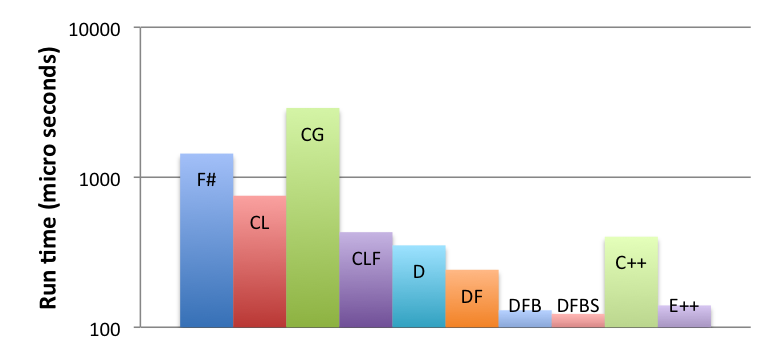
\includegraphics[width=\columnwidth]{results/micro_add3_runtime.png}
\subcaption{Runtime performance comparison of different approaches on adding three vectors of 100 elements for one million times.}
\label{fig:runtime_add3}
\end{subfigure}
\hfill
\begin{subfigure}[b]{.58\textwidth}
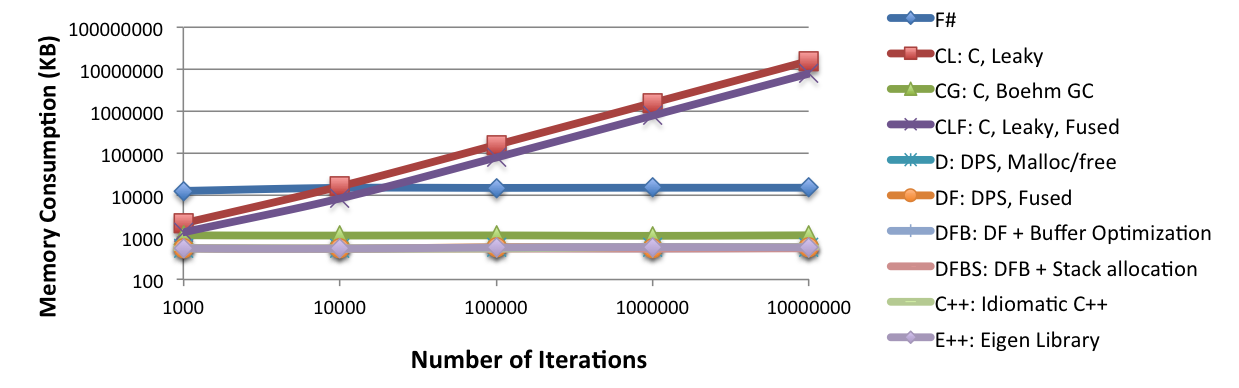
\includegraphics[width=\columnwidth]{results/micro_add3_mem.png}
\subcaption{Memory consumption comparison of different approaches on adding three vectors of 100 elements by varying the number of iterations. All the invisible lines are hidden under the bottom line.}
\label{fig:mem_add3}
\end{subfigure}
\begin{subfigure}[b]{.38\textwidth}
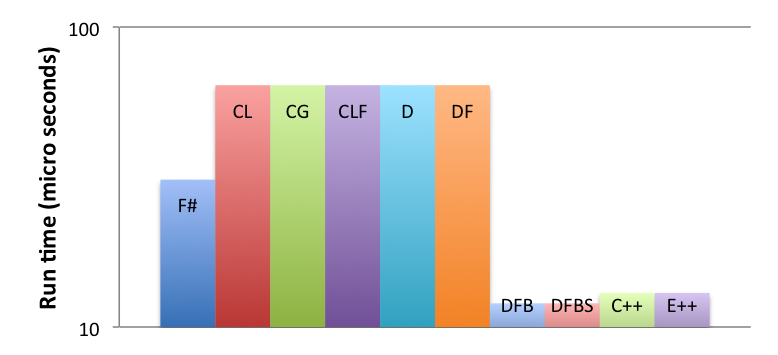
\includegraphics[width=\columnwidth]{results/micro_cross_runtime.png}
\subcaption{Runtime performance comparison of different approaches on cross product of two vectors of three elements for one million times.}
\label{fig:runtime_cross}
\end{subfigure}
\hfill
\begin{subfigure}[b]{.58\textwidth}
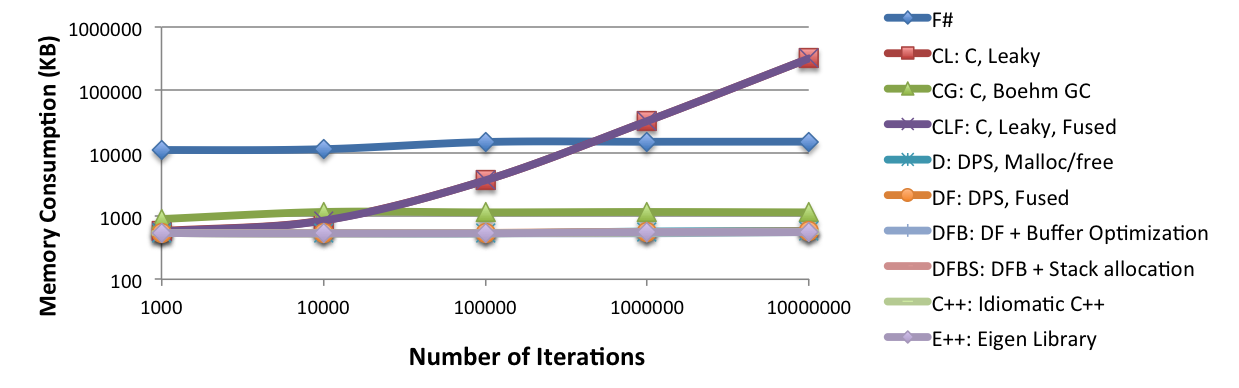
\includegraphics[width=\columnwidth]{results/micro_cross_mem.png}
\subcaption{Memory consumption comparison of different approaches on cross product of two vectors of three elements by varying the number of iterations.}
\label{fig:mem_cross}
\end{subfigure}
\caption{Experimental Results for Micro Benchmarks}
\label{fig:exp_micro}
\end{figure*}

Throughout this section, we compare the performance and memory consumption of the following alternatives:

%\def\apara#1{\noindent{\bf #1}}
\def\apara#1{\item {\bf #1}}
\begin{itemize}
\apara{F\#:} Using the array operations (e.g. map) provided in the standard library of F\# to implement vector operations.

\apara{CL: Leaky C code}, which is the generated C code from \lafsharp{}, using malloc to allocate vectors, never calling free.
\apara{CG: C code using Boehm GC}, which is the generated C code from \lafsharp{}, using \cod{GC\_malloc} of Boehm GC to allocate vectors.

\apara{CLF: CL + Fused Loops}, performs deforestation and loop fusion before CL.

\apara{D: DPS C code using system-provided malloc/free}, translates \lafsharp{} programs into \salafsharp{} before generating C code. Hence, the generated C code frees all allocated vectors. In this variant, the malloc and free functions are used for memory management.

\apara{DF: D + Fused Loops}, which is similar to the previous one, but performs deforestation before translating to \salafsharp{}. 
\apara{DFB: DF + Buffer Optimizations}, which performs the buffer optimizations described in Section~\ref{sec_simplification} 
(such as allocation hoisting and merging) on \salafsharp{} expressions. 

\apara{DFBS: DFB using stack allocator}, same as DFB, but using bump allocation for memory management, as previously discussed in Section~\ref{sec:ccodegen}.
This is the best C code we generate from \lafsharp{}.

\apara{C++: Idiomatic C++}, which uses an handwritten C++ vector library, depending on C++14 move construction and copy elision for performance, with explict programmer indication of fixed-size (known at compile time) vectors, permitting stack allocation.

\apara{E++: Eigen C++}, which uses the Eigen~\cite{guennebaud2010eigen} library which is implemented using C++ expression templates to effect loop fusion and copy elision. Also uses explicit sizing for fixed-size vectors.
\end{itemize}

First, we investigate the behavior of several variants of generated C code for two micro benchmarks. More specifically we see how DPS improves both performance and memory consumption in comparison with an F\# version. The behavior of the generated DPS code is very similar to manually handwritten C++ code and the Eigen library.

Then, we demonstrate the benefit of using DPS for some real-life computer vision and machine learning workloads motivated in~\cite{srajerbenchmark}. Based on the results for these workloads, we argue that using DPS is a great choice for generating C code for numerical workloads, such as computer vision algorithms, running on embedded devices with a limited amount of memory available. 
\subsection{Micro Benchmarks}

Figure~\ref{fig:exp_micro} shows the experimental results for micro benchmarks, one adding three vectors, the second using vector cross product.



\paragraph{add3}: vectorAdd(vectorAdd(vec1, vec2), vec3)\\ 
in which all the vectors contain 100 elements. This program is run one million times in a loop, and timing results are shown in Figure~\ref{fig:runtime_add3}.
In order to highlight the performance differences, the figure uses a logarithmic scale on its Y-axis. Based on these results we make the following observations.
First, we see that all C and C++ programs are outperforming the F\# program, except the one which uses the Boehm GC.
This shows the overhead of garbage collection in the F\# runtime environment and Boehm GC.
Second, loop fusion has a positive impact on performance. This is because this program involves creating an intermediate vector (the one resulting from addition of vec1 and vec2). 
Third, the generated DPS C code which uses buffer optimizations (DFB) is faster than the one without this optimization (DF). 
This is mainly because the result vector is allocated only once for DFB whereas it is allocated once per iteration in DF. Finally, there is no clear advantage for C++ versions.  This is mainly due to the fact that the vectors have sizes not known at compile time, hence the elements are not stack allocated. The Eigen version partially compensates this limitation by using vectorized operations, making the performance comparable to our best generated DPS C code.

The peak memory consumption of this program for different approaches is shown in Figure~\ref{fig:mem_add3}. This measurement is performed by running this program by varying number of iterations. Both axes use logarithmic scales to better demonstrate the memory consumption difference. As expected, F\# uses almost the same amount of memory over the time, due to garbage collection. However, the runtime system sets the initial amount to 15MB by default. Also unsurprisingly, leaky C uses memory linear in the number of iterations, albeit from a lower base.  The fused version of leaky C (CLF) decreases the consumed memory by a constant factor. Finally, DPS C, and C++ use a constant amount of space which is one order of magnitude less than the one used by the F\# program, and half the amount used by the generated C code using Boehm GC.


\begin{figure*}[t]
\begin{subfigure}[t]{.38\textwidth}
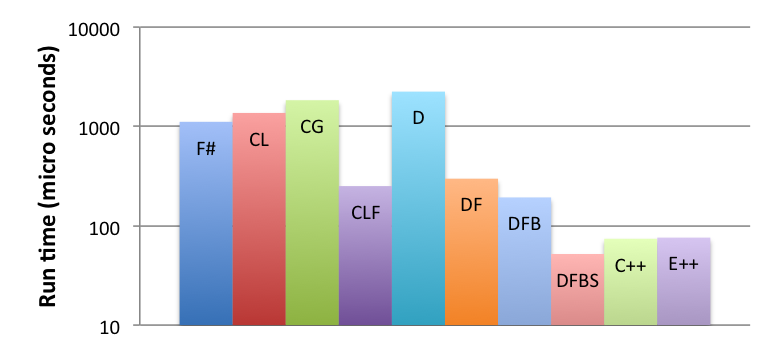
\includegraphics[width=\columnwidth]{results/proj_runtime.png}
\subcaption{Runtimes: Bundle Adjustment}
\label{fig:runtime_ba}
\end{subfigure}
\hfill
\begin{subfigure}[t]{.58\textwidth}
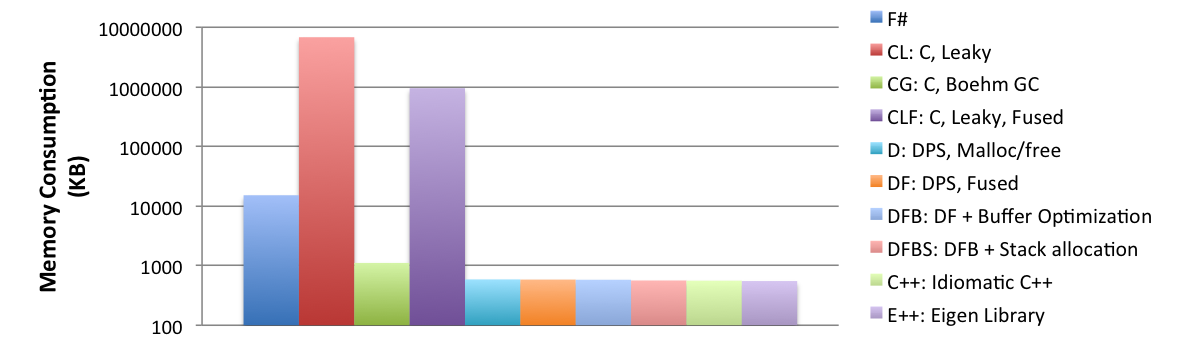
\includegraphics[width=\columnwidth]{results/proj_mem.png}
\subcaption{Memory consumption: Bundle Adjustment}
\label{fig:mem_ba}
\end{subfigure}
\begin{subfigure}[t]{.38\textwidth}
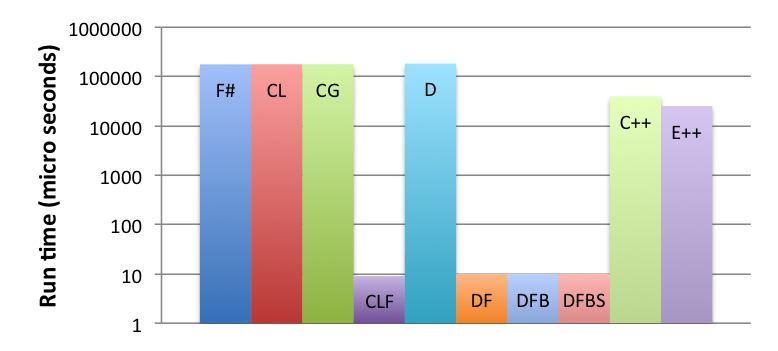
\includegraphics[width=\columnwidth]{results/gmm_runtime.png}
\subcaption{Runtimes: GMM}
\label{fig:runtime_gmm}
\end{subfigure}
\hfill
\begin{subfigure}[t]{.58\textwidth}
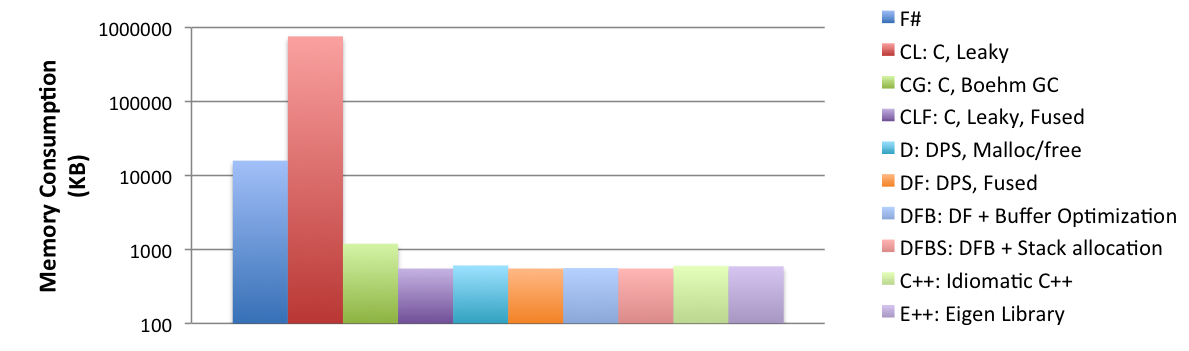
\includegraphics[width=\columnwidth]{results/gmm_mem.png}
\subcaption{Memory consumption: GMM}
\label{fig:mem_gmm}
\end{subfigure}
\begin{subfigure}[t]{.38\textwidth}
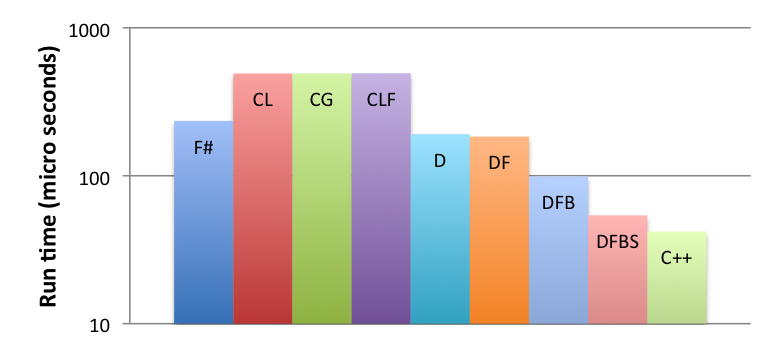
\includegraphics[width=\columnwidth]{results/ht_runtime.png}
\subcaption{Runtimes: Hand Tracking}
\label{fig:runtime_ht}
\end{subfigure}
\hfill
\begin{subfigure}[t]{.58\textwidth}
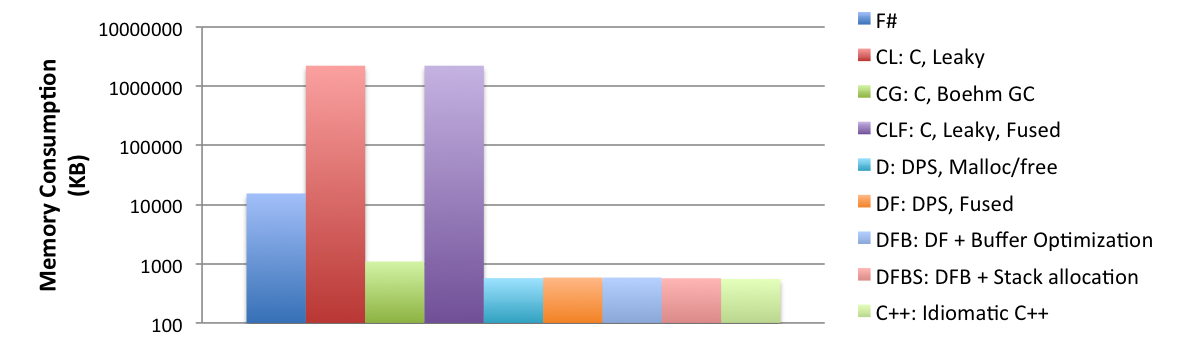
\includegraphics[width=\columnwidth]{results/ht_mem.png}
\subcaption{Memory consumption: Hand Tracking}
\label{fig:mem_ht}
\end{subfigure}
\caption{Experimental Results for Computer Vision and Machine Learning Workloads}
\end{figure*}

\paragraph{cross}: vectorCross(vec1, vec2)\\
This micro-benchmark is 1 million runs in which the two vectors contain 3 elements.  Timing results are in Figure~\ref{fig:runtime_cross}. 
We see that the F\# program is faster than the generated leaky C code, perhaps because garbage collection is invoked less frequently than in \emph{add3}. Overall, in both cases, the performance of F\# program and generated leaky C code is very similar.
In this example, loop fusion does not have any impact on performance, as the program contains only one operator. 
As in the previous benchmark, all variants of generated DPS C code have a similar performance and outperform the generated leaky C code and the one using Boehm GC, for the same reasons.
Finally, both handwritten and Eigen C++ programs have a similar performance to our generated C programs. For the case of this program, both C++ libraries provide fixed-sized vectors, which results in stack allocating the elements of the two vectors. This has a positive impact on performance. Furthermore, as there is no SIMD version of the cross operator, we do not observe a visible advantage for Eigen.

Finally, we discuss the memory consumption experiments of the second program, which is shown in Figure~\ref{fig:mem_cross}. This experiment leads to the same observation as the one for the first program. However, as the second program does not involve creating any intermediate vector, loop fusion does not improve the peak memory consumption.

The presented micro benchmarks show that our DPS generated C code improves both performance and memory consumption by an order of magnitude in comparison with an equivalent F\# program. 
Also, the generated DPS C code promptly deallocates memory which makes the peak memory consumption constant over the time, as opposed to a linear increase of memory consumption of the generated leaky C code. In addition, by using bump allocators the generated DPS C code can improve performance as well. 
Finally, we see that the generated DPS C code behaves very similarly to both handwritten and Eigen C++ programs.

Next, we investigate the performance and memory consumption of real-life workloads.

\subsection{Computer Vision and Machine Learning Workloads}
\paragraph{Bundle Adjustment} \cite{triggs1999bundle} is a  computer vision problem which has many applications. In this problem, the goal is to optimize several parameters in order to have an accurate estimate of the projection of a 3D point by a camera. This is achieved by minimizing an objective function representing the reprojection error.  This objective function is passed to a nonlinear minimizer as a function handle, and is typically called many times during the minimization.

One of the core parts of this objective function is the \emph{project} function which is responsible for finding the projected coordinates of a 3D point by a camera, including a model of the radial distortion of the lens. The \lafsharp{} implementation of this method is given in Figure~\ref{fig:ba_code}.
\begin{figure}[t]
\hfill\begin{minipage}{.75\textwidth}\raggedright
\lett{} radialDistort = \vabs{(radical: Vector) (proj: Vector)}{}\\
\tabt \lett{} rsq = vectorNorm proj\\
\tabt \lett{} L = 1.0 + radical.[0] * rsq + radical.[1] * rsq * rsq\\
\tabt vectorSMul proj L\\
\lett{} rodriguesRotate = \vabs{(rotation: Vector) (x: Vector)}{}\\
\tabt \lett{} sqtheta = vectorNorm rotation\\
\tabt \cod{if} sqtheta != 0. \cod{then}\\
\tabt\tabt \lett{} theta = sqrt sqtheta\\
\tabt\tabt \lett{} thetaInv = 1.0 / theta\\
\tabt\tabt \lett{} w = vectorSMul rotation thetaInv\\
\tabt\tabt \lett{} wCrossX = vectorCross w x\\
\tabt\tabt \lett{} tmp = (vectorDot w x) * (1.0 - (cos theta))\\
\tabt\tabt \lett{} v1 = vectorSMul x (cos theta)\\
\tabt\tabt \lett{} v2 = vectorSMul wCrossX (sin theta) \\
\tabt\tabt vectorAdd (vectorAdd v1 v2) (vectorSMul w tmp)\\
\tabt \cod{else} \\
\tabt\tabt vectorAdd x (vectorCross rotation x)\\
\lett{} project = \vabs{(cam: Vector) (x: Vector)}{}\\
\tabt\lett{} rotation = vectorSlice cam 0 2 \\
\tabt\lett{} center = vectorSlice cam 3 5 \\
\tabt\lett{} radical = vectorSlice cam 9 10 \\
\tabt\lett{} Xcam =  \\
\tabt\tabt rodriguesRotate rotation (vectorSub x center) \\
\tabt\lett{} distorted =  \\
\tabt\tabt radialDistort radical ( \\
\tabt\tabt \tabt vectorSMul ( \\
\tabt\tabt \tabt \tabt vectorSlice Xcam 0 1 \\
\tabt\tabt \tabt ) (1.0/Xcam.[2])) \\
\tabt vectorAdd (vectorSlice cam 7 8) ( \\
\tabt\tabt vectorSMul distorted cam.[6] \\
\tabt  )
\end{minipage}\hfill
\caption{Bundle Adjustment functions in \lafsharp{}.}
\label{fig:ba_code}
\end{figure}

Figure~\ref{fig:runtime_ba} shows the runtime of different approaches after running \emph{project} ten million times. First, the F\# program performs similarly to the leaky generated C code and the C code using Boehm GC. Second, loop fusion improves speed fivefold. Third, the generated DPS C code is slower than the generated leaky C code, mainly due to costs associated with intermediate deallocations. However, this overhead is reduced by using bump allocation and performing loop fusion and buffer optimizations. Finally, we observe that the best version of our generated DPS C code marginally  outperforms both C++ versions.

The peak memory consumption of different approaches for Bundle Adjustment is shown in Figure~\ref{fig:mem_ba}. First, the F\# program uses three orders of magnitude less memory in comparison with the generated leaky C code, which remains linear in the number of calls. This improvement is four orders of magnitude in the case of the generated C code using
Boehm GC. Second, loop fusion improves the memory consumption of the leaky C code by an order of magnitude, due to removing several intermediate vectors. Finally, all generated DPS C variants as well as C++ versions consume the same amount of memory. The peak memory consumption of is an order of magnitude better than the F\# baseline. 

\paragraph{The Gaussian Mixture Model} is a workhorse machine learning tool, used for computer vision applications such as image background modelling and image denoising, as well as semi-supervised learning. 

In GMM, loop fusion can successfully remove all intermediate vectors. Hence, there is no difference between CL and CLF, or between DS and DSF, 
in terms of both performance and peak memory consumption as can be observed in Figure~\ref{fig:runtime_gmm} and Figure~\ref{fig:mem_gmm}. Both C++ libraries do not support the loop fusion needed for GMM. Hence, they behave three orders of magnitude worse than our fused and DPS generated C code.

Due to the cost for performing memory allocation (and deallocation for DPS) at each iteration, the F\# program, the leaky C code, and the generated DPS C code exhibit a worse performance than the fused and stack allocated versions. Furthermore, as the leaky C code does not deallocate the intermediate vectors, it monotonically increases the consumed memory.

\paragraph{Hand tracking} is a computer vision/computer graphics workload~\cite{taylor2014user} that includes matrix-matrix multiplies, and numerous combinations of fixed- and variable-sized vectors and matrices.
Figure~\ref{fig:runtime_ht} shows performance results of running one of the main functions of hand-tracking for 1 million times. As in the \emph{cross} micro-benchmark we see no advantage for loop fusion, because in this function the intermediate vectors have multiple consumers. Similar to previous cases generating DPS C code improves runtime performance, which is improved even more by using bump allocation and performing loop fusion and buffer optimizations. However, in this case the idiomatic C++ version outperforms the generated DPS C code. Figure~\ref{fig:mem_ht} shows that DPS generated programs consume an order of magnitude less memory than the F\# baseline, equal to the C++ versions.


\section{Related Work}
\label{sec:related}
\subsection{Programming Languages without GC}
Functional programming languages without using garbage collection dates back to Linear Lisp~\cite{baker1992lively}. However, most functional languages (dating back to
the Lisp around 1959) use garbage collection for managing memory.

Region-based memory management was first introduced in ML~\cite{TOFTE1997109} and then in an extended version of C, called Cyclone~\cite{Grossman:2002:RMM:512529.512563}, as an alternative or complementary technique to in order to remove the need for runtime garbage collection. This is achieved by allocating memory regions based on the liveness of objects. This approach improves both performance and memory consumption in many cases. However, in many cases the size of the regions is not known, whereas in our approach the size of each storage location is computed using the shape expressions. Also, in practice there are cases in which one needs to combine this technique with garbage collection~\cite{Hallenberg:2002:CRI:512529.512547}, as well as cases in which the performance is still not satisfying~\cite{Birkedal:1996:RIV:237721.237771, Tofte:2004:RRM:993034.993040}. Furthermore, the complexity of region inference, hinders the maintenance of the compiler, in addition to the overhead it causes for compilation time.

Safe~\cite{montenegro2009simple, montenegro2008type} suggests a simpler region inference algorithm by restricting the language to a first-order functional language. Also, linear regions~\cite{fluet2006linear} relax the stack discipline restriction on region-based memory management. This is because of certain usecases, which use unbounded amount of memory due to recursion. A Haskell implementation of this approach is given in~\cite{kiselyov2008lightweight}. The restricted form of recursion allowed by \lafsharp{} means that we never face similar issues. Hence, we choose to always follow the stack discipline for memory management.

\subsection{Estimation of Memory Consumption}

One can use type systems for estimating memory consumption. Hofmann and Jost \cite{Hofmann:2003:SPH:604131.604148} enrich the type system with certain annotations and uses linear programming for the heap consumption inference. Another approach is to use sized types~\cite{vasconcelos2008space} for the same purpose.

Size slicing~\cite{Henriksen:2014:SSH:2636228.2636238} uses a technique similar to ours for inferring the shape of arrays in the Futhark programming language. However, in \lafsharp{} we guarantee that shape inference is simplified and is based only on size computation, whereas in their case, they rely on compiler optimizations for its simplification and in some cases it can fall back to inefficient approaches which in the worst case could be as expensive as evaluating the original expression~\cite{Hofmann:2003:SPH:604131.604148}. The FISh programming language~\cite{jay1999programming} also makes shape information explicit in programs, and resolves the shapes at compilation time by using partial evaluation.

Clinger~\cite{Clinger98propertail} explores different space efficiency classes. Based on the proposed formalism he defines formally what it means for a language to \textit{properly} handle tail recursion. Next, we see related work on optimizing tail recursive calls.

\subsection{Optimizing Tail Calls}
Destination-passing style was originally introduced in~\cite{larus1989restructuring}, then was encoded functionally in~\cite{Research98afunctional} by using linear types~\cite{turner1995once, wadler1990linear}. Walker and Morrisett \cite{walker2000alias} use extensions to linear type systems to support aliasing which is avoided in vanilla linear type systems. The idea of destination-passing style has many similarities to \textit{tail-recursion modulo cons}~\cite{friedman1975unwinding, wadler1984listlessness}.

\subsection{Array Programming Languages}
APL~\cite{iverson1962programming} can be considered as the first array programming language. Futhark~\cite{Henriksen:2014:SSH:2636228.2636238, Henriksen:2014:BCI:2627373.2627388} and SAC~\cite{Grelck2006} are functional array programming languages. One interesting property of such languages is the support for fusion, which is achieved in \lafsharp{} by certain rewrite rules. However, as this topic is out of the scope of this paper, we leave more discussion for the future work.

There are many domain-specific languages (DSLs) for numerical workloads such as Opt~\cite{devito2016opt}, 
Halide~\cite{ragan2013halide}, Diderot~\cite{chiw2012diderot}, and OptiML~\cite{sujeeth2011optiml}. All these DSLs 
generate parallel code from their high-level programs. 
Furthermore, Halide~\cite{ragan2013halide}
exploits the memory hierarchy by making tiling and scheduling decisions, similar to Spiral~\cite{spiral} and LGen~\cite{spampinato2016basic}. 
Although both parallelism and improving use of a memory
hierarchy are orthogonal concepts to translation into DPS, they are still interesting directions for \lafsharp{}.  


\begin{small}
\bibliographystyle{abbrvnat}
\bibliography{ref} 
\end{small}

% \bibliographystyle{abbrvnat}

% % The bibliography should be embedded for final submission.

% \begin{thebibliography}{}
% \softraggedright

% \bibitem[Smith et~al.(2009)Smith, Jones]{smith02}
% P. Q. Smith, and X. Y. Jones. ...reference text...

% \end{thebibliography}
\end{document}
